% !TEX program = pdflatex
% SAHAY-AI research report: references, trained model, training and evaluation.
% Build: pdflatex (run twice for the table of contents and cross-references).
\documentclass[11pt,a4paper]{article}

\usepackage[T1]{fontenc}
\usepackage[utf8]{inputenc}
\usepackage{lmodern}
\usepackage[a4paper,margin=2.2cm,headheight=14pt]{geometry}
\usepackage{microtype}
\usepackage{amsmath,amssymb}
\usepackage{booktabs,tabularx,array,multirow}
\usepackage[table]{xcolor}

\definecolor{sahayblue}{HTML}{1F4E79}
\definecolor{sahaygreen}{HTML}{2E7D32}
\definecolor{sahayred}{HTML}{B3261E}
\definecolor{sahayorange}{HTML}{D97706}
\definecolor{sahaygray}{HTML}{5F6368}
\definecolor{sahaypurple}{HTML}{6A3D9A}
\definecolor{selrow}{HTML}{E8F0F8}

\usepackage{caption}
\captionsetup{font=small,labelfont={bf,color=sahayblue},skip=4pt}
\usepackage{enumitem}
\setlist{itemsep=2pt,topsep=4pt,parsep=0pt}
\usepackage{pgfplots}
\pgfplotsset{compat=1.18}
\usepackage{tikz}
\usetikzlibrary{positioning,arrows.meta,calc}
\usepackage{tcolorbox}
\tcbuselibrary{skins,breakable}
\usepackage{fancyhdr}
\usepackage{float}
\usepackage{titlesec}
\usepackage{needspace}
% Keep a section heading with at least a few lines of its body.
\newcommand{\sectionbreak}{\needspace{10\baselineskip}}
\titleformat{\section}{\Large\bfseries\color{sahayblue}}{\thesection}{0.6em}{}
\titleformat{\subsection}{\large\bfseries\color{sahayblue!85!black}}{\thesubsection}{0.5em}{}
\titleformat{\subsubsection}{\normalsize\bfseries}{\thesubsubsection}{0.5em}{}
\usepackage[colorlinks=true,linkcolor=sahayblue,citecolor=sahaygreen,urlcolor=sahayblue]{hyperref}
\urlstyle{same}

% Float placement: allow more floats per text page and stack float-only pages from the top.
\renewcommand{\topfraction}{0.9}
\renewcommand{\bottomfraction}{0.8}
\renewcommand{\textfraction}{0.07}
\renewcommand{\floatpagefraction}{0.75}
\setcounter{topnumber}{3}
\setcounter{totalnumber}{5}
\makeatletter
\setlength{\@fptop}{0pt}
\setlength{\@fpsep}{14pt plus 4pt}
\setlength{\@fpbot}{0pt plus 1fil}
\makeatother

\pagestyle{fancy}
\fancyhf{}
\fancyhead[L]{\small\color{sahaygray}SAHAY-AI --- Research report v1.0}
\fancyhead[R]{\small\color{sahaygray}Development evidence only --- not clinical, not official}
\fancyfoot[C]{\small\thepage}
\renewcommand{\headrulewidth}{0.4pt}

\newcommand{\pass}{\textcolor{sahaygreen}{\textbf{pass}}}
\newcommand{\fail}{\textcolor{sahayred}{\textbf{fail}}}
\newcommand{\na}{\textcolor{sahaygray}{n/a}}
% Typewriter identifiers that may break after underscores; \filepath breaks paths at / . _ -
\newcommand{\codeus}{\textunderscore\allowbreak}
\DeclareRobustCommand{\code}[1]{{\ttfamily\let\_\codeus #1}}
\DeclareUrlCommand\filepath{\urlstyle{tt}}
\newcommand{\evA}{\textsf{\textbf{A}}}
\newcommand{\evB}{\textsf{\textbf{B}}}
\newcommand{\evC}{\textsf{\textbf{C}}}
\newcommand{\evD}{\textsf{\textbf{D}}}

\newtcolorbox{keybox}[1][]{enhanced,breakable,colback=sahayblue!4,colframe=sahayblue,
  boxrule=0.6pt,arc=2pt,left=6pt,right=6pt,top=4pt,bottom=4pt,fonttitle=\bfseries\small,#1}
\newtcolorbox{warnbox}[1][]{enhanced,breakable,colback=sahayred!4,colframe=sahayred,
  boxrule=0.6pt,arc=2pt,left=6pt,right=6pt,top=4pt,bottom=4pt,fonttitle=\bfseries\small,#1}

\pgfplotsset{
  sahay/.style={
    tick label style={font=\scriptsize},
    label style={font=\footnotesize},
    legend style={font=\scriptsize,draw=sahaygray!50},
    grid=major, grid style={sahaygray!20},
  }
}

\hypersetup{
  pdftitle={SAHAY-AI: Literature Foundations, Experimental Shadow Classifier and Evaluation Report},
  pdfauthor={SAHAY-AI AI/ML and Safety workstream},
  pdfsubject={NHAA 14566 - Problem Statement 26093 - research report},
}

\begin{document}

\pagenumbering{alph}
%======================================================================
\begin{titlepage}
\centering
{\small\color{sahaygray} National Helpline Against Atrocities (NHAA, 14566) \textbullet{} Problem Statement 26093 \textbullet{} Ministry of Social Justice and Empowerment\par}
\vspace{2.4cm}
{\fontsize{34}{40}\selectfont\bfseries\color{sahayblue} SAHAY-AI\par}
\vspace{0.5cm}
{\LARGE Literature Foundations, Experimental Shadow Classifier\\[2pt] and Evaluation Report\par}
\vspace{0.9cm}
{\large Research report \textbullet{} Version 1.0 \textbullet{} 13 September 2026\par}
\vspace{1.6cm}
\begin{warnbox}[title={What this report is, and what it is not}]
\small
\begin{itemize}
  \item Every model number here is \textbf{development evidence}. It is either synthetic
        (fictional records from a template generator) or \emph{contaminated} regression on
        fixtures whose outcomes have already been published. None is an official, independent,
        blind, locked or clinical result. \textbf{The locked evaluation set holds 0 samples.}
  \item The trained model, \code{experimental\_shadow\_classifier}, has the status
        \code{rejected\_for\_product\_integration}. It runs only in an operator-run local CLI
        demonstration, beside the deterministic pipeline, which remains the authority.
  \item SAHAY-AI does not diagnose PTSD, depression or any other condition. It claims no clinical
        validity, calibration or production readiness.
\end{itemize}
\end{warnbox}
\vfill
{\small\color{sahaygray} Prepared by the SAHAY-AI AI/ML and Safety workstream. Sources: the repository
(\code{ml/}, \code{docs/}), the private training root (\code{sih-dataset/}), and the eight references in the
bibliography, each verified online on 13 September 2026.\par}
\end{titlepage}
\pagenumbering{roman}

%======================================================================
\begin{abstract}
\noindent SAHAY-AI is a bounded, human-in-the-loop intake and triage prototype for India's National
Helpline Against Atrocities (NHAA, 14566). This report does three things. First, it reviews the eight
references that ground the project: speech-based PTSD and emotion detection, the helpline's
operational mandate, India's data-protection law, a multilingual encoder for Indian languages, open
speech recognition, and a Hindi counselling-dialogue emotion corpus. Second, it documents the one
machine-learning model the team trained: an eight-label multilingual \emph{shadow} classifier built
on MuRIL. The encoder was domain-adapted with masked-language modelling on 512{,}605 external text
windows, then supervised on fictional, template-generated SAHAY records. Third, it reports every
evaluation that was performed, keeping each evidence class separate.

Domain adaptation reduced held-out masked-language perplexity from 11.95 to 6.17. The Task~7
checkpoint reached micro-F1 0.78 on its synthetic development test, but crisis recall on validation
was only 0.23. On the exposed regression fixtures it lagged the deterministic lexicon pipeline:
micro-F1 0.67 against 0.91 on dev, over the seven shared labels. A targeted hardening round
(Task~7B) raised crisis recall on a frozen synthetic holdout to 1.00 in English, Hindi and Hinglish.
It still missed the pre-registered macro-F1 gate (0.675 against 0.70), cut continuing-threat
recall to 0.11, and could not be evaluated on three labels that had no positive holdout support.
It also did worse than Task~7 on the exposed fixtures. Both checkpoints therefore remain rejected
for product integration.

The deterministic pipeline remains the authority. After safety hardening it misses 1 of 17
critical events on the dev fixtures and 1 of 14 on the (now exposed) candidate fixtures, and it
passes all 39 exposed guardrail red-team cases. The report closes with limitations and a concrete
path to an independent evaluation.
\end{abstract}

\vspace{0.4cm}
\tableofcontents
\newpage
\pagenumbering{arabic}

%======================================================================
\section{Introduction}

\subsection{Operational context}
The Ministry of Social Justice and Empowerment (MoSJE) runs the National Helpline Against Atrocities
(NHAA) on the toll-free number 14566~\cite{pib2021}. The helpline supports enforcement of the
Protection of Civil Rights (PCR) Act, 1955 and the Scheduled Castes and Scheduled Tribes (Prevention
of Atrocities) Act, 1989. It is available around the clock across the country, in Hindi, English and
the regional languages of the States and UTs.

Problem Statement 26093 (MoSJE) asks for an \emph{``AI-enabled Real-Time Stress and
Trauma Assessment Module''} that assesses stress, trauma, fear, anxiety and vulnerability across NHAA
channels. It names voice and text analysis, a vulnerability index with Low/Moderate/High/Critical
bands, detection of suicidal ideation and intimidation, recommended support pathways, and multilingual
operation under privacy and consent constraints.

\subsection{The SAHAY-AI design stance}
SAHAY-AI treats that brief as a \emph{bounded intake instrument}, not a counsellor or a diagnostic
tool:
\begin{itemize}
  \item A deterministic 12-state dialogue machine chooses every approved intent. A language model
        may only phrase that intent, and a validator checks every sentence before it is spoken.
  \item A synchronous crisis pre-check runs before dialogue policy on every utterance. A match
        forces the fixed crisis script, Critical priority and a human takeover.
  \item A deterministic Stress Vulnerability Index (SVI) combines nine evidence-linked dimensions,
        D1--D9. It abstains (\code{needs\_human}) when confidence is low.
  \item A human executive decides every action. The victim never sees any score, band, alert or
        confidence.
\end{itemize}
These are the project's non-negotiable safety invariants. The model in this report is judged against
them: it may only \emph{add evidence beside} the deterministic pipeline, never replace it.

\subsection{Why train a model at all?}
The deterministic detectors are precise, but they are brittle to paraphrase, indirect wording and
code-switching. Before hardening, they missed 4 of 14 critical events on the candidate fixtures
(\S\ref{sec:det}). A learned multilingual encoder is the natural complement, but only if it can be
\emph{shown} to help. The team therefore trained it strictly in shadow mode, under a pre-registered
selection and promotion protocol. The protocol is authorised by decision EXT-119 and its Invariant~8
clarification.

\subsection{Evidence classes}
Every number in this report belongs to exactly one of four evidence classes. They are never pooled
(Table~\ref{tab:evidence}).

\begin{table}[!htbp]
\centering\small
\caption{Evidence classes used throughout the report.}
\label{tab:evidence}
\begin{tabularx}{\linewidth}{@{}>{\raggedright\arraybackslash}p{2.7cm}>{\raggedright\arraybackslash}p{4.3cm}X@{}}
\toprule
Class & What it is & What it can and cannot support \\
\midrule
\evA{} External auxiliary & Masked-language perplexity and source-namespace auxiliary metrics on external datasets & Evidence of language modelling only. \emph{Never} a SAHAY safety metric: source labels such as subreddit, stress, emotion, sentiment or hate speech are not SAHAY labels. \\
\evB{} Synthetic development & Metrics on fictional records from the same template generator (validation, \code{synthetic\_development\_test}, the Task~7B frozen holdout) & Shows the model learned the generator's patterns. Says \emph{nothing} about real speech or text. \\
\evC{} Contaminated regression & The published dev, candidate and red-team fixtures, run once after selection & A regression check next to the deterministic pipeline. Never used for training, early stopping, thresholds or selection. \\
\evD{} Official / independent & The locked set and the human-authored blind corpus & \textbf{Empty}: the locked count is 0 and nothing has been frozen, so no official number exists. \\
\bottomrule
\end{tabularx}
\end{table}

\subsection{Structure}
Section~\ref{sec:lit} reviews the eight references. Section~\ref{sec:system} summarises the system.
Section~\ref{sec:data} describes the data, and Section~\ref{sec:model} the model and its training.
Section~\ref{sec:eval} reports all evaluations. Sections~\ref{sec:discussion}--\ref{sec:next}
discuss findings, limitations and next steps. The appendices hold the provenance hashes and the
label definitions.

%======================================================================
\section{Literature and reference review}
\label{sec:lit}

The eight references fall into five themes. For each one we summarise the verified facts, say how it
bears on SAHAY-AI, and appraise it critically. All details were checked against the publisher,
abstract or repository page on 13 September 2026.

\subsection{Speech markers of PTSD and emotion}

\paragraph{Hu et al.\ (2024)~\cite{hu2024}.} \emph{Speech-based recognition and estimating severity of
PTSD using machine learning}, Journal of Affective Disorders 362:859--868. The authors recorded
speech from \textbf{76 patients with PTSD and 60 controls}. They extracted acoustic features with
the openSMILE toolkit and selected features with a random forest. Classifiers on an 18-feature set
gave strong binary results: the random-forest model reached \textbf{accuracy 0.975} and \textbf{AUC 1.0}.
A regression model predicting PCL-5 severity scores was statistically significant, but weak
(\textbf{MSE 0.90, MAE 0.76, $R^2 = 0.10$}, $p<0.001$). The authors themselves note that feature
selection may inflate the results, that the underlying mechanisms are unexplained, and that the
regression needs validation on larger datasets.

\paragraph{Islam and ElSayed (2024)~\cite{islam2024}.} \emph{Speech-Based Emotion Recognition and PTSD
Detection through Machine and Deep Learning}, IJCERT 11(3):46--53. The study combined the acted
RAVDESS emotional-speech corpus with PTSD-specific recordings, after noise reduction. It extracted
acoustic and temporal features and compared SVMs and random forests against CNNs and LSTMs. Deep
models reached \textbf{up to 91\% accuracy for emotion recognition} and \textbf{89\% for PTSD
detection}, clearly ahead of the classical models. The authors flag limited generalisability across
populations and obstacles to real-world deployment.

\paragraph{Critical appraisal.}
Both studies show that acoustic signals carry information about trauma-related states, but three
cautions apply before carrying their numbers over to a helpline:
\begin{itemize}
  \item \textbf{Small or acted samples.} With 136 speakers, an AUC of exactly 1.0 is a warning sign
        of selection optimism, which the authors acknowledge. RAVDESS is acted, scripted English
        speech; acted emotion is not the spontaneous distress of a first-contact call in Hindi or
        Hinglish.
  \item \textbf{Weak severity signal.} $R^2 = 0.10$ means acoustic features explain about a tenth
        of the variance in symptom severity. That argues \emph{against} deriving a severity score
        from voice.
  \item \textbf{Provenance.} The source of the PTSD recordings in~\cite{islam2024} is not described
        in its abstract, so the result cannot be reproduced from the paper's summary alone.
\end{itemize}

\paragraph{Implications for SAHAY-AI.}
The two studies motivate SVI dimension D4, \emph{acute distress (acoustic and emotional)}, weight 0.12.
SAHAY-AI deliberately treats it as a distress \emph{indicator}, never as a diagnosis. The output
validator rejects any assistant sentence that names PTSD, trauma, depression or a disorder as fact.
D4 is also currently \textbf{structurally unavailable}: no approved, usable acoustic corpus exists.
The local CREMA-D copy consists of Git LFS pointers, and RAVDESS (EXT-003) and Common Voice Hindi
(EXT-002) are still only proposed. The SVI therefore renormalises over the remaining 0.88 of weight
on text sessions. The high headline accuracies in~\cite{hu2024,islam2024} are also why this report
insists on denominators, undefined-metric handling and separate evidence classes.

\subsection{Operational mandate: NHAA 14566}
The MoSJE press release of December 2021~\cite{pib2021} gives these facts about the helpline:
\begin{itemize}
  \item toll-free number \textbf{14566}, operating round the clock nationwide;
  \item reachable by voice call or VOIP from any mobile or landline operator, and through a
        web-based self-service portal;
  \item Hindi, English and the regional languages of the States and UTs;
  \item a \textbf{docket number for every complaint}, with online status tracking;
  \item the goal of making sure the victim-related provisions of the PoA Act, 1989 and the PCR Act,
        1955 are complied with, from complaint registration and FIR through to investigation and
        charge-sheeting within statutory timelines;
  \item awareness-building about those legal provisions.
\end{itemize}

\noindent These features map directly onto SAHAY-AI. The multilingual mandate drives the Hindi,
English and Hinglish MVP. Docketing and tracking become the status-only \emph{victim timeline}. The
statutory-compliance goal drives the legal-urgency dimension (D8) and the escalation packet.
SAHAY-AI does not integrate with the live helpline: that needs departmental approval, an authorised
operator and DLT registration.

\subsection{Legal framework: DPDP Act 2023 and Rules 2025}
The Digital Personal Data Protection Act, 2023 (Act~22 of 2023, assented in August 2023) is India's
general data-protection law~\cite{meity2023}. MeitY notified the implementing \emph{DPDP Rules, 2025} in mid-November
2025; sources give 13 or 14 November. Commencement is phased over 18 months:
\begin{itemize}
  \item the Data Protection Board provisions took effect immediately;
  \item the consent-manager provisions follow after 12 months (around November 2026);
  \item most substantive obligations follow after 18 months (around May 2027).
\end{itemize}
Those substantive obligations cover notice and consent, reasonable security safeguards, breach
intimation to the Board and to affected Data Principals, verifiable parental consent for children's
data, retention limits and erasure, and extra duties for Significant Data Fiduciaries. Penalties
reach INR~250~crore.

\begin{table}[!htbp]
\centering\small
\caption{How DPDP principles map to SAHAY-AI controls (design alignment only; not legal advice).}
\label{tab:dpdp}
\begin{tabularx}{\linewidth}{@{}>{\raggedright\arraybackslash}p{4.2cm}X@{}}
\toprule
DPDP principle & SAHAY-AI control (MVP) \\
\midrule
Notice and informed consent & Consent gate with AI disclosure before any capture; scoring suppressed if consent is declined; ``Talk to a person'' always visible. \\
Purpose limitation, minimisation & Victim clients never receive the SVI, bands, dimensions, alerts or confidence (enforced server-side and tested); queue previews minimised. \\
Security safeguards & All speech and NLP runs locally; audio never leaves the deployment; role-filtered event fan-out; no keys in the repository. \\
Retention and erasure & Audio kept for less time than derived case data; the training artefacts have a documented keep, quarantine and delete policy. \\
Children's data & The external training datasets carry a \code{minors\_possible} flag; they stay quarantined research artefacts and never reach the product. \\
Breach intimation, Board & \emph{Not implemented.} A production deployment would need a breach process and a legal review. \\
\bottomrule
\end{tabularx}
\end{table}

\noindent Separately, the licensing and privacy status of the external training datasets is
\textbf{unresolved} (\S\ref{sec:data}). EXT-119 records a project-owner risk acceptance for private,
local research only. It is not a lawful-basis determination.

\subsection{Multilingual text representation: MuRIL}
MuRIL (Khanuja et al., Google Research India, arXiv:2103.10730)~\cite{khanuja2021} is a BERT-base encoder pre-trained
only on Indian-language text:
\begin{itemize}
  \item \textbf{17 languages}: 16 Indian languages plus English;
  \item \textbf{236M parameters}, a \textbf{197{,}285-token vocabulary}, sequences of up to 512
        tokens, and about 16B unique training tokens;
  \item two objectives: masked-language modelling (MLM) on monolingual text and translation-language
        modelling (TLM) on parallel data;
  \item data from Common Crawl (OSCAR) and Wikipedia, translated pairs (PMINDIA and in-house
        translations) and transliterated pairs (Dakshina, indic-trans);
  \item low-resource languages upsampled with exponent $\alpha = 0.3$.
\end{itemize}
On XTREME-style tasks MuRIL beat mBERT with an average of \textbf{68.6 vs 59.1} on native-script test
sets and \textbf{48.9 vs 21.1} on transliterated test sets.

\paragraph{Why SAHAY-AI uses it.} Helpline text mixes Devanagari Hindi, English and \emph{romanised}
Hinglish. MuRIL's large advantage on transliterated input is exactly the property we need. Our own
runtime qualification (\S\ref{sec:runtime}) found that the pinned MuRIL tokeniser uses about 23\%
fewer tokens per character than XLM-R on Hindi (0.246 vs 0.319) and about 12\% fewer on Hinglish
(0.259 vs 0.294), with a 0\% unknown-token rate. Our Stage~A sampler reuses MuRIL's upsampling
exponent $\alpha=0.3$, applied across source datasets instead of languages (\S\ref{sec:stageA}).

\subsection{Speech recognition: IndicConformer and faster-whisper}
\paragraph{IndicConformer~\cite{ai4bharat}.} AI4Bharat's IndicConformer is a suite of open ASR models
covering all \textbf{22 official Indian languages}. The multilingual model has \textbf{600M
parameters} and uses hybrid RNN-Transducer models built on the Conformer architecture. It is
released under the MIT licence through Hugging Face and a direct object store. In SAHAY-AI it is the
\emph{roadmap} path to the 22 scheduled languages. It has no external-dependency approval, has
\textbf{not been downloaded}, and no WER has been measured with it.

\paragraph{faster-whisper~\cite{systran}.} SYSTRAN's faster-whisper reimplements OpenAI Whisper on
the CTranslate2 inference engine. It is up to 4$\times$ faster than the reference implementation at
the same accuracy, uses less memory, supports 8-bit quantisation on CPU and GPU, and integrates
Silero VAD (MIT licence). Its README benchmark for the \emph{small} model on CPU shows why int8
matters for a laptop fallback:
\begin{itemize}
  \item fp32, beam 5: 2\,min~37\,s and 2{,}257\,MB RAM;
  \item int8, beam 5: 1\,min~42\,s and 1{,}477\,MB, about 35\% less time and memory;
  \item int8 with batch 8: 51\,s and 3{,}608\,MB.
\end{itemize}
SAHAY-AI runs Whisper Small through faster-whisper~1.2.1 and CTranslate2~4.8.2. The official
checkpoint was converted locally to CTranslate2 fp16 on the GPU, with a CPU int8 fallback labelled
\emph{degraded}. The \emph{only} application entry point is Silero VAD gating (\S\ref{sec:runtime}).

\subsection{Hindi emotion in counselling dialogue: EmoInHindi}
EmoInHindi (Singh, Priya, Firdaus, Ekbal and Bhattacharyya, IIT Patna; LREC 2022,
pp.~5829--5837)~\cite{singh2022} contains \textbf{1{,}814 dialogues} and \textbf{44{,}247 utterances}. They were created in a
Wizard-of-Oz manner \emph{for mental-health and legal counselling of crime victims}. Each utterance
carries one or more of 16 emotion labels (including neutral) and an intensity. The paper also
proposes contextual baselines for emotion and intensity recognition.

\paragraph{Relevance and use.} EmoInHindi is the public resource closest to SAHAY-AI's domain:
Hindi, crime-victim, counselling-style dialogue. Under EXT-119 it was used only for Stage~A
masked-language modelling (10{,}815 coverage windows, 14.6\% of continuation draws) and for an
\emph{isolated} Stage~B auxiliary head (\S\ref{sec:stageB}). Its emotion labels are never mapped to
D4 (which is acoustic), the SVI, a band or crisis. The publisher permits research use only and does
not address redistribution, so the dataset stays \code{licence\_pending}. One local observation is
unreconciled: the processed local copy exposes 17 label names (Stage~B vocabulary size 17), while
the paper states 16.

\subsection{Synthesis}
\begin{table}[!htbp]
\centering\footnotesize
\caption{The eight references: verified findings, role in SAHAY-AI, and current status.}
\label{tab:refs}
\begin{tabularx}{\linewidth}{@{}c>{\raggedright\arraybackslash}p{2.6cm}>{\raggedright\arraybackslash}X>{\raggedright\arraybackslash}p{3.3cm}>{\raggedright\arraybackslash}p{3.0cm}@{}}
\toprule
\# & Reference & Key verified finding & Role in SAHAY-AI & Status in project \\
\midrule
1 & Hu et al.\ 2024~\cite{hu2024} & 76 PTSD / 60 controls; openSMILE features + RF; acc.\ 0.975, AUC 1.0; PCL-5 regression $R^2$ 0.10 & Motivates the D4 acoustic channel; argues against voice-derived severity & Not reproduced; D4 unavailable \\
2 & Islam \& ElSayed 2024~\cite{islam2024} & RAVDESS + PTSD recordings; deep models up to 91\% (emotion), 89\% (PTSD) & Speech emotion as an auxiliary signal only; acted-speech caveat & Not reproduced; RAVDESS not approved \\
3 & MoSJE / PIB~\cite{pib2021} & NHAA 14566: 24$\times$7, toll-free, multilingual; docket and tracking; PCR / PoA Acts & Deployment context, timeline, D8 legal urgency & Context only; no live integration \\
4 & MeitY DPDP~\cite{meity2023} & Consent, notice, safeguards, breach, children; Rules 2025 phased to 2027 & Privacy-by-design controls (Table~\ref{tab:dpdp}) & Alignment documented; legal review pending \\
5 & Khanuja et al.\ 2021~\cite{khanuja2021} & 17 languages, 236M params, MLM+TLM; translit.\ 48.9 vs mBERT 21.1 & Base encoder of the trained shadow classifier & Used (rev.\ \code{afd9f36c}, Apache-2.0) \\
6 & AI4Bharat~\cite{ai4bharat} & IndicConformer 600M, 22 languages, Conformer hybrid RNNT, MIT & Roadmap ASR for 22 languages & Not downloaded; not benchmarked \\
7 & SYSTRAN~\cite{systran} & CTranslate2 Whisper, up to 4$\times$ faster, int8, Silero VAD & ASR runtime for Whisper Small & Used (v1.2.1, VAD-gated) \\
8 & Singh et al.\ 2022~\cite{singh2022} & 1{,}814 WoZ dialogues, 44{,}247 utterances, 16 labels + intensity; crime-victim counselling & Hindi domain text for Stage A / B & Used under EXT-119; licence pending \\
\bottomrule
\end{tabularx}
\end{table}

%======================================================================
\section{System context}
\label{sec:system}

Figure~\ref{fig:arch} places the trained model inside the SAHAY-AI architecture. It has two paths.
The \emph{reply path} is synchronous and protected by the crisis pre-check. The \emph{assessment
path} runs in parallel and never blocks a reply. The shadow classifier sits entirely outside both
decision paths.

\begin{figure}[!htbp]
\centering
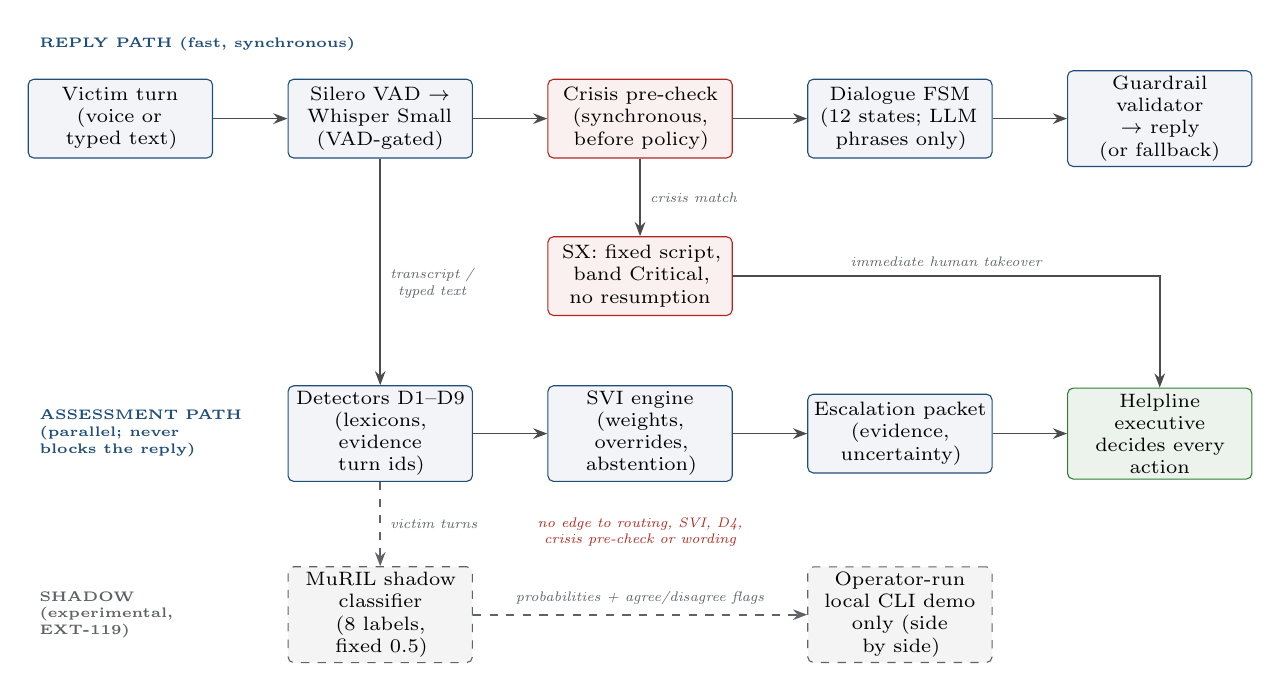
\begin{tikzpicture}[
  box/.style={draw=sahayblue, rounded corners=2pt, fill=sahayblue!6, align=center, font=\scriptsize,
              minimum height=10mm, text width=22mm, inner sep=2pt},
  crit/.style={box, draw=sahayred, fill=sahayred!7},
  hum/.style={box, draw=sahaygreen, fill=sahaygreen!9},
  shd/.style={box, draw=sahaygray, dashed, fill=sahaygray!7},
  arr/.style={-{Stealth[length=1.8mm]}, semithick, draw=black!70},
  darr/.style={arr, dashed, draw=sahaygray},
  lab/.style={font=\tiny\itshape, text=sahaygray, align=center},
  plabel/.style={font=\tiny\bfseries, text=sahayblue, align=left, anchor=west},
]
\node[box]  (in)  at (0,0)     {Victim turn\\(voice or typed text)};
\node[box]  (asr) at (3.3,0)   {Silero VAD $\rightarrow$\\Whisper Small\\(VAD-gated)};
\node[crit] (pre) at (6.6,0)   {Crisis pre-check\\(synchronous,\\before policy)};
\node[box]  (fsm) at (9.9,0)   {Dialogue FSM\\(12 states; LLM\\phrases only)};
\node[box]  (val) at (13.2,0)  {Guardrail validator\\$\rightarrow$ reply\\(or fallback)};
\node[crit] (sx)  at (6.6,-2.0) {SX: fixed script,\\band Critical,\\no resumption};
\node[box]  (det) at (3.3,-4.0)  {Detectors D1--D9\\(lexicons, evidence\\turn ids)};
\node[box]  (svi) at (6.6,-4.0)  {SVI engine\\(weights, overrides,\\abstention)};
\node[box]  (pkt) at (9.9,-4.0)  {Escalation packet\\(evidence,\\uncertainty)};
\node[hum]  (exe) at (13.2,-4.0) {Helpline executive\\decides every\\action};
\node[shd]  (shw) at (3.3,-6.3)  {MuRIL shadow\\classifier\\(8 labels, fixed 0.5)};
\node[shd]  (cli) at (9.9,-6.3)  {Operator-run\\local CLI demo\\only (side by side)};

\draw[arr] (in) -- (asr);
\draw[arr] (asr) -- (pre);
\draw[arr] (pre) -- (fsm);
\draw[arr] (fsm) -- (val);
\draw[arr] (pre) -- node[lab, right] {crisis match} (sx);
\draw[arr] (sx.east) -- node[lab, above, pos=0.5] {immediate human takeover} (sx.east -| exe.north) -- (exe.north);
\draw[arr] (asr) -- node[lab, right, pos=0.55] {transcript /\\typed text} (det);
\draw[arr] (det) -- (svi);
\draw[arr] (svi) -- (pkt);
\draw[arr] (pkt) -- (exe);
\draw[darr] (det) -- node[lab, right] {victim turns} (shw);
\draw[darr] (shw) -- node[lab, above] {probabilities + agree/disagree flags} (cli);
\node[lab, text=sahayred] at (6.6,-5.25) {no edge to routing, SVI, D4,\\crisis pre-check or wording};
\node[plabel] at (-1.15,0.95) {REPLY PATH (fast, synchronous)};
\node[plabel] at (-1.15,-4.0) {ASSESSMENT PATH\\(parallel; never\\blocks the reply)};
\node[plabel, text=sahaygray] at (-1.15,-6.3) {SHADOW\\(experimental,\\EXT-119)};
\end{tikzpicture}
\caption{SAHAY-AI architecture and where the trained model sits. Solid arrows are authoritative paths;
dashed arrows are shadow-only. The deterministic pipeline runs unchanged with every model absent.}
\label{fig:arch}
\end{figure}

\paragraph{The Stress Vulnerability Index.} The SVI is a deterministic weighted sum,
$\mathrm{SVI} = \sum_i w_i\, s_i$, with each dimension score $s_i \in [0,100]$
(Table~\ref{tab:svi}). The bands are Low (0--29), Moderate (30--54), High (55--74) and Critical
(75--100). \emph{Hard overrides} sit outside the sum: a confirmed D1 (immediate danger) or D2
(crisis) forces Critical, and confidence below 0.45, poor audio or low language confidence yields
\code{needs\_human} with \emph{no score}. On typed channels D4 is structurally unavailable, so the
weights renormalise over the remaining 0.88.

\begin{table}[!htbp]
\centering\small
\caption{SVI dimensions and provisional weights (pending expert calibration).}
\label{tab:svi}
\begin{tabular}{@{}llc@{\hspace{0.6cm}}llc@{}}
\toprule
Dim & Meaning & Weight & Dim & Meaning & Weight \\
\midrule
D1 & Immediate safety threat & 0.22 & D6 & Isolation, boycott, displacement & 0.08 \\
D2 & Crisis / self-harm language & 0.18 & D7 & Medical urgency & 0.08 \\
D3 & Fear, intimidation, threats & 0.13 & D8 & Legal urgency & 0.06 \\
D4 & Acute distress (acoustic, emotional) & 0.12 & D9 & Communication safety & 0.05 \\
D5 & Trauma-associated indicators & 0.08 & & & \\
\bottomrule
\end{tabular}
\end{table}

\paragraph{The eight detector categories.} Both the deterministic pipeline and the shadow model are
scored on the same schema. It has eight multi-label categories: crisis / self-harm, immediate
danger, continuing threat, medical urgency, isolation / boycott / displacement, legal urgency,
communication-safety coercion, and explicit human request (definitions in Appendix~\ref{app:labels}).
The deterministic pipeline has no text detector for \emph{explicit human request}, because the app
sends that request from a button. Deterministic metrics therefore cover seven categories.

%======================================================================
\section{Data}
\label{sec:data}

\subsection{External corpora (Stage A and B only)}
EXT-119 authorised local, offline training on every usable, privacy-processed text record of five
external datasets (Table~\ref{tab:ext}). All five remain \code{licence\_pending}, and every output is
a \code{quarantined\_research\_artifact}. The builder counts blank rows, unreadable bytes and LFS
pointers but never invents them. Text is split into windows of at most 480 characters on word or
turn boundaries, so each fits a 128-token input.

\begin{table}[!htbp]
\centering\footnotesize
\caption{External datasets used for encoder adaptation (Stage A) and isolated auxiliary heads (Stage B).
$^{\ast}$Dialogues. $^{\dagger}$15{,}000 labelled records plus 3{,}199 unlabelled ones used for MLM only.}
\label{tab:ext}
\begin{tabularx}{\linewidth}{@{}>{\raggedright\arraybackslash}p{3.3cm}>{\raggedright\arraybackslash}p{2.2cm}rrr>{\raggedright\arraybackslash}X@{}}
\toprule
Dataset & Language / script & Records & Windows & Dup.\ recs & Stage B auxiliary task (source namespace) \\
\midrule
Reddit Suicide Detection & English & 232{,}072 & 466{,}055 & 519 & Subreddit membership (not a clinical judgement) \\
Dreaddit & English & 715 & 968 & 0 & Annotated stress (not crisis) \\
EmoInHindi~\cite{singh2022} & Hindi (mostly mixed script) & 1{,}814$^{\ast}$ & 10{,}861 & 4 & Multi-label emotion (not severity) \\
Hinglish hate-speech (local derivative) & Romanised & 18{,}199$^{\dagger}$ & 20{,}151 & 2{,}912 & Hate-speech label (not threat or danger) \\
Hinglish sentiment & Romanised Hinglish & 14{,}569 & 14{,}570 & 684 & None: classes 0/1/2 are opaque \\
CREMA-D & --- & 0 & --- & --- & Unavailable: all 22{,}326 media files are Git LFS pointers \\
\midrule
\textbf{Total} & & \textbf{267{,}369} & \textbf{512{,}605} & & 263{,}904 duplicate families \\
\bottomrule
\end{tabularx}
\end{table}

\paragraph{Governance.}
\begin{itemize}
  \item Every window is weighted by $1/\text{family size}$, so near-duplicates do not dominate.
  \item About 0.5\% of families are held out as \code{mlm\_validation} and about 10\% form an
        auxiliary test bucket. No family crosses partitions.
  \item The privacy pass redacts URLs, e-mail addresses, phone numbers, long numbers and social
        handles. Examples: 11{,}556 Reddit records were redacted, and 955 EmoInHindi records.
        Rule-based redaction \emph{cannot} catch names or contextual identifiers.
  \item A \textbf{source-label firewall} refuses every automatic mapping from a source label to a
        SAHAY concept. For example: stress $\not\to$ crisis, subreddit of origin $\not\to$ routing,
        sentiment $\not\to$ SVI, emotion $\not\to$ D4, hate speech $\not\to$ continuing threat,
        and ``non-suicide'' $\not\to$ safe.
\end{itemize}

\subsection{Fictional SAHAY corpus (Task 7, Stage C)}
The SAHAY head was supervised \emph{only} on private fictional records. They come from a committed
bank of \textbf{110 templates} in English, Devanagari Hindi and romanised Hinglish:
\begin{itemize}
  \item \textbf{Size:} 6{,}605 records, split \emph{by template} into 5{,}005 train, 757 validation
        and 843 \code{synthetic\_development\_test}.
  \item \textbf{Coverage:} single- and multi-turn records, multi-label cases, safe and low-distress
        controls, expected-abstention cases and human-help requests. Also negation, quotation,
        attribution, past events, indirect and conditional wording, misspellings, Unicode variants
        and code-switching.
  \item \textbf{Contamination screen:} every rendered variant was checked against the exposed
        fixtures. Hits (39 shared distinctive phrases, 8 high token overlaps) blocked \textbf{5
        template families} (115 records). Blocked families were left out, never reworded to evade
        the check.
\end{itemize}

\subsection{Targeted hardening corpus (Task 7B, \code{7b-v1})}
An ID-only error analysis of the Task~7 checkpoint found crisis misses concentrated in Hindi and
Hinglish, especially in conditional (``temporal ambiguity''), indirect and ``disappear'' wording.
It also found coercion confused with ordinary disagreement, and legal help confused with legal
urgency. A targeted corpus answered this:
\begin{itemize}
  \item \textbf{Families:} 105 fictional cores with explicit contrast families. Direct framings
        keep their label; quoted, reported, past and negated framings flip it.
  \item \textbf{Size:} 9{,}924 records: 35\% English, 28\% Hindi, 38\% Hinglish.
  \item \textbf{Focus areas:} crisis 34\%, coercion 21\%, legal 19\%, multi-label 13\%, other 14\%.
  \item \textbf{Freeze:} the corpus was frozen and hashed \emph{before} training
        (2026-09-12 11:01:49 IST).
  \item \textbf{Review packet:} 2{,}266 items across 718 families were prepared, but
        \textbf{0 human reviews are complete}.
\end{itemize}

\begin{table}[!htbp]
\centering\footnotesize
\caption{Task 7B split sizes and positive label support. Three labels have \emph{no} positives in either validation or holdout.}
\label{tab:7bsupport}
\setlength{\tabcolsep}{3.8pt}
\begin{tabular}{@{}lrrrrrrrrrr@{}}
\toprule
Split & Records & Families & Crisis & Imm.\ dgr & Cont.\ thr & Medical & Isolation & Legal & Coercion & Human req. \\
\midrule
Train & 7{,}492 & 634 & 2{,}108 & 268 & 453 & 254 & 246 & 1{,}200 & 1{,}441 & 370 \\
Validation & 1{,}242 & 42 & 318 & \textbf{0} & 243 & \textbf{0} & \textbf{0} & 212 & 236 & 105 \\
Holdout & 1{,}190 & 42 & 298 & \textbf{0} & 132 & \textbf{0} & \textbf{0} & 209 & 216 & 118 \\
\bottomrule
\end{tabular}
\end{table}

\subsection{Deterministic evaluation corpora}
Label schema 1.0.0 defines these corpora, all of them fictional:
\begin{itemize}
  \item \textbf{dev:} 57 samples (13 Hindi, 28 English, 16 Hinglish); tuning allowed;
  \item \textbf{candidate:} 48 samples (12 Hindi, 22 English, 14 Hinglish); never tuned on, but
        every outcome has been published, so the split is exposed;
  \item \textbf{locked:} \textbf{0 samples}, because no fixture has the required real reviewer
        approvals;
  \item \textbf{red-team:} 39 guardrail cases, plus 75 near-miss cases and 29 urgency-leakage
        cases written during hardening, plus 8 red-team \emph{victim-input} cases.
\end{itemize}
A blind-evaluation harness exists (\code{ml/eval/blind/}). Its \code{run} command refuses with exit
code~12 because no corpus has been frozen.

%======================================================================
\section{Model and training}
\label{sec:model}

\subsection{Architecture}
\code{experimental\_shadow\_classifier} is built from four parts:
\begin{itemize}
  \item \textbf{Encoder:} MuRIL-base, pinned at revision \code{afd9f36c}~\cite{khanuja2021}: 12
        layers, hidden size 768, 12 attention heads, feed-forward size 3{,}072, vocabulary 197{,}285.
        It was domain-adapted in Stage~A.
  \item \textbf{Pooling:} attention-masked mean pooling, then dropout 0.1.
  \item \textbf{Head:} one linear layer with \textbf{8 independent logits} (sigmoid,
        BCE-with-logits), no routing, SVI, D4, diagnosis or generative head.
  \item \textbf{Input and threshold:} victim turns only, joined in order, truncated to 128 tokens.
        The decision threshold is fixed at an \textbf{uncalibrated 0.5} and never tuned.
\end{itemize}
Training used PyTorch 2.11.0+cu128 and Transformers 5.17.0 on a single laptop RTX~4060 (8\,GB),
fully offline with sockets blocked (0 network attempts recorded).

\subsection{Stage A: domain-adaptive masked-language modelling}
\label{sec:stageA}
Stage~A continues MuRIL's MLM objective on the external corpus in two phases:
\begin{enumerate}
  \item a seeded \emph{coverage pass} of 277{,}185 training windows, so every usable record
        contributes at least its first window;
  \item a \emph{balanced continuation} of 40{,}000 windows, each dataset drawn with probability
        proportional to its window count raised to the power 0.3. MuRIL uses the same exponent for
        language upsampling~\cite{khanuja2021}; here it is applied across datasets.
\end{enumerate}
The continuation cut the suicide corpus to 45.0\% of draws. Hinglish hate speech took 17.5\%,
Hinglish sentiment 15.9\%, EmoInHindi 14.6\% and Dreaddit 7.0\%; Dreaddit's small pool was cycled
through four passes.

\begin{table}[!htbp]
\centering\small
\caption{Stage A configuration and results (evidence class \evA).}
\label{tab:stageA}
\begin{tabularx}{\linewidth}{@{}>{\raggedright\arraybackslash}p{5.8cm}X@{}}
\toprule
Setting & Value \\
\midrule
Masking & Dynamic 15\% (80\% \code{[MASK]}, 10\% random, 10\% unchanged); loss on masked tokens, weighted by duplicate family \\
Optimiser, schedule & AdamW (fused), learning rate $5\times10^{-5}$, weight decay 0.01, 6\% warmup then linear decay, gradient clip 1.0 \\
Batch, length, precision, seed & Micro-batch 32, 128 tokens, bf16 autocast with fp32 master weights, seed 20260912 \\
Optimiser steps, wall time & 9{,}913 (8{,}663 coverage + 1{,}250 continuation); 3{,}606\,s ($\approx$\,60\,min) at $\approx$\,91 windows/s \\
Peak GPU memory & 5{,}923\,MB allocated, 9{,}134\,MB reserved (above the 8\,GB of dedicated VRAM, so it spilled into shared memory); max 57\,$^\circ$C \\
\midrule
\textbf{Validation loss / perplexity} (2{,}732 windows, 33{,}197 masked tokens) & before: 2.480 / \textbf{11.945}; after coverage: 1.854 / 6.385; after continuation: 1.819 / \textbf{6.165} ($-48.4\%$ perplexity) \\
\bottomrule
\end{tabularx}
\end{table}

\begin{figure}[!htbp]
\centering
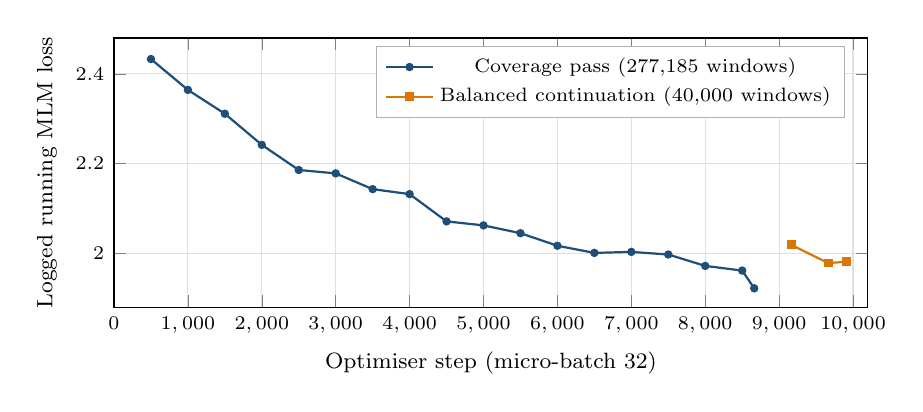
\begin{tikzpicture}
\begin{axis}[sahay, width=0.92\linewidth, height=5.0cm,
  xlabel={Optimiser step (micro-batch 32)}, ylabel={Logged running MLM loss},
  xmin=0, xmax=10200, ymin=1.88, ymax=2.48, scaled x ticks=false,
  xticklabel style={/pgf/number format/1000 sep={,}},
  legend pos=north east]
\addplot[sahayblue, thick, mark=*, mark size=1.1pt] coordinates {
  (500,2.4331) (1000,2.3643) (1500,2.3112) (2000,2.2418) (2500,2.1858) (3000,2.1782)
  (3500,2.1431) (4000,2.1320) (4500,2.0712) (5000,2.0623) (5500,2.0449) (6000,2.0169)
  (6500,2.0010) (7000,2.0032) (7500,1.9974) (8000,1.9720) (8500,1.9616) (8663,1.9220)};
\addlegendentry{Coverage pass (277{,}185 windows)}
\addplot[sahayorange, thick, mark=square*, mark size=1.2pt] coordinates {
  (9163,2.0190) (9663,1.9784) (9913,1.9812)};
\addlegendentry{Balanced continuation (40{,}000 windows)}
\end{axis}
\end{tikzpicture}
\caption{Stage A training loss from the run console. The small step up at the start of the continuation
most likely reflects the shift in data mix toward the smaller Hinglish, Hindi and Dreaddit sources.}
\label{fig:stageA}
\end{figure}

\noindent A 2{,}048-window smoke run was done first (perplexity 14.03 $\to$ 10.37 on its smaller
validation set). It is not used.

\subsection{Stage B: isolated auxiliary heads}
\label{sec:stageB}
Stage~B trained one head per source dataset on the Stage~A encoder. Labels were kept in their source
namespace (\code{source:<dataset>:<value>}), with at most 12{,}000 training and 3{,}000 test windows
per source. It is a diagnostic of what the adapted encoder represents. Its checkpoint
\textbf{never} initialised or touched the SAHAY head. Hinglish sentiment was excluded because its
classes are opaque.

\begin{table}[!htbp]
\centering\small
\caption{Stage B source-namespace results (evidence class \evA; not SAHAY safety metrics).}
\label{tab:stageB}
\setlength{\tabcolsep}{5pt}
\begin{tabular}{@{}llrrccc@{}}
\toprule
Source & Task & Train win. & Test win. & Micro F1 & Macro F1 & Exact match \\
\midrule
Reddit Suicide Detection & 2-class & 12{,}000 & 3{,}000 & 0.900 & 0.890 & 0.900 \\
Hinglish hate speech & 2-class & 12{,}000 & 1{,}652 & 0.827 & 0.824 & 0.827 \\
Dreaddit & 2-class & 860 & 108 & 0.657 & 0.644 & 0.657 \\
EmoInHindi & multi-label (17) & 9{,}783 & 1{,}078 & 0.667 & 0.355 & 0.049 \\
\bottomrule
\end{tabular}
\end{table}

\noindent On EmoInHindi the head reaches F1 0.88 on \emph{anticipation} and 0.83 on \emph{joy}.
It \textbf{never predicts} 7 of the 17 labels: annoyed, apprehensive, confused, \emph{fear}, guilty,
impressed and surprised, all with F1~0.00. Fear (210 test positives) is exactly the emotion a
helpline cares about, which illustrates why emotion labels are not a usable proxy for distress.

\subsection{Stage C: the SAHAY shadow head (Task 7)}
Stage~C starts from the Stage~A encoder and trains the eight-label head on the fictional corpus.
Settings:
\begin{itemize}
  \item AdamW (fused); encoder learning rate $3\times10^{-5}$, head learning rate $10^{-3}$;
  \item linear schedule with 6\% warmup; micro-batch 32; bf16; gradient clip 1.0;
  \item BCE-with-logits loss; seeds 13, 42 and 97.
\end{itemize}
Two runs are disclosed:
\begin{itemize}
  \item \textbf{Run~1:} at most 6 epochs, patience 2. It hit the epoch cap while validation was
        still improving, so early stopping never acted.
  \item \textbf{Run~2:} at most 20 epochs, patience 3, everything else identical. It is the one
        change that lets the declared early-stopping rule actually decide.
\end{itemize}
The rule, fixed before training, ranks candidates on \emph{validation only}:
\begin{enumerate}
  \item higher validation macro F1;
  \item higher minimum per-label recall;
  \item lower validation loss;
  \item lower seed, then earlier run.
\end{enumerate}

\begin{table}[!htbp]
\centering\footnotesize
\caption{Stage C candidates (evidence class \evB). Selection used validation columns only; synthetic-test columns are shown for transparency. The selected row is shaded.}
\label{tab:stageC}
\begin{tabular}{@{}llcccccccc@{}}
\toprule
& & & \multicolumn{4}{c}{Validation (757)} & \multicolumn{3}{c}{Synthetic dev.\ test (843)} \\
\cmidrule(lr){4-7}\cmidrule(l){8-10}
Run & Seed & Epoch (of run) & Macro F1 & Min.\ label R & Crisis R & Loss & Macro F1 & Micro F1 & Crisis R \\
\midrule
1 & 13 & 6 (6) & 0.437 & 0.013 & 0.013 & 0.284 & 0.532 & 0.672 & 0.111 \\
1 & 42 & 6 (6) & 0.428 & 0.000 & 0.091 & 0.293 & 0.514 & 0.659 & 0.181 \\
1 & 97 & 6 (6) & 0.321 & 0.007 & 0.026 & 0.353 & 0.353 & 0.588 & 0.042 \\
2 & 13 & 15 (18) & 0.609 & 0.197 & 0.325 & 0.454 & \textbf{0.806} & \textbf{0.806} & \textbf{0.500} \\
2 & 42 & 10 (13) & 0.630 & 0.104 & 0.260 & 0.428 & 0.732 & 0.763 & 0.417 \\
\rowcolor{selrow} 2 & 97 & 9 (12) & \textbf{0.645} & \textbf{0.234} & 0.234 & 0.373 & 0.761 & 0.783 & 0.458 \\
\bottomrule
\end{tabular}
\end{table}

\noindent Three observations follow from Table~\ref{tab:stageC}:
\begin{itemize}
  \item \textbf{Loss and F1 disagree.} Run~1 has a \emph{lower} validation loss than Run~2 but far
        lower macro F1. With imbalanced multi-label BCE, predicting mostly negatives is cheap in
        loss, so F1-first selection was the right call.
  \item \textbf{Seed variance is large.} Run~2 synthetic-test macro F1 spans 0.73--0.81 across
        seeds. Differences under about 0.05 should not be read as real.
  \item \textbf{Validation and test disagree.} Seed 13 is best on the synthetic test, but the rule
        correctly chose from validation only. The two splits also differ in difficulty: validation
        holds 142 \emph{conditional}-wording records and 153 \emph{indirect} ones, while the test
        split has no conditional records. That is why validation crisis recall (0.23) is half the
        test value (0.46).
\end{itemize}

\begin{figure}[!htbp]
\centering
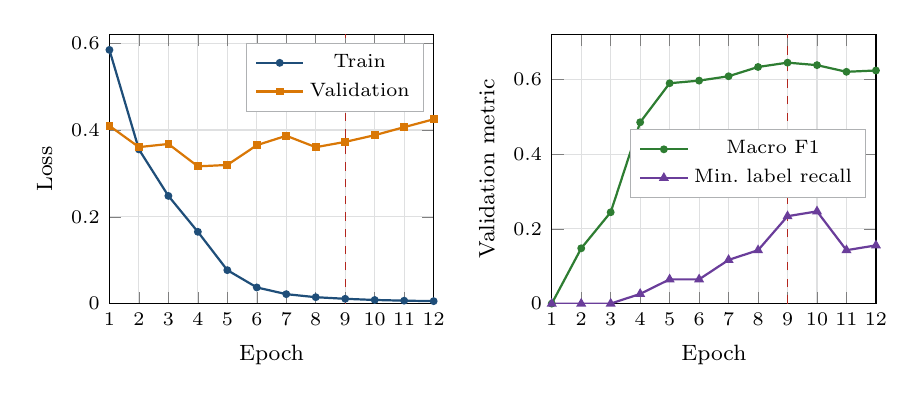
\begin{tikzpicture}
\begin{axis}[sahay, name=left, width=0.47\linewidth, height=5.0cm,
  xlabel={Epoch}, ylabel={Loss}, xmin=1, xmax=12, ymin=0, ymax=0.62, xtick={1,...,12},
  legend style={at={(0.97,0.97)}, anchor=north east}]
\addplot[sahayblue, thick, mark=*, mark size=1pt] coordinates {
  (1,0.5844)(2,0.3552)(3,0.2481)(4,0.1654)(5,0.0771)(6,0.0373)(7,0.0218)(8,0.0148)
  (9,0.0111)(10,0.0084)(11,0.0068)(12,0.0057)};
\addlegendentry{Train}
\addplot[sahayorange, thick, mark=square*, mark size=1pt] coordinates {
  (1,0.40951)(2,0.36049)(3,0.36776)(4,0.31619)(5,0.3194)(6,0.36493)(7,0.38665)(8,0.36033)
  (9,0.37256)(10,0.38797)(11,0.40647)(12,0.42462)};
\addlegendentry{Validation}
\draw[sahayred, dashed] (axis cs:9,0) -- (axis cs:9,0.62);
\end{axis}
\begin{axis}[sahay, at={(left.east)}, anchor=west, xshift=1.5cm, width=0.47\linewidth, height=5.0cm,
  xlabel={Epoch}, ylabel={Validation metric}, xmin=1, xmax=12, ymin=0, ymax=0.72, xtick={1,...,12},
  legend style={at={(0.97,0.52)}, anchor=east}]
\addplot[sahaygreen, thick, mark=*, mark size=1pt] coordinates {
  (1,0.0)(2,0.148)(3,0.2444)(4,0.4851)(5,0.5895)(6,0.5965)(7,0.6082)(8,0.633)
  (9,0.6446)(10,0.6379)(11,0.6201)(12,0.6236)};
\addlegendentry{Macro F1}
\addplot[sahaypurple, thick, mark=triangle*, mark size=1.3pt] coordinates {
  (1,0)(2,0)(3,0)(4,0.026)(5,0.0649)(6,0.0649)(7,0.1169)(8,0.1429)
  (9,0.2338)(10,0.2468)(11,0.1429)(12,0.1558)};
\addlegendentry{Min.\ label recall}
\draw[sahayred, dashed] (axis cs:9,0) -- (axis cs:9,0.72);
\end{axis}
\end{tikzpicture}
\caption{Selected Task 7 run (Run 2, seed 97). The validation loss bottoms out at epoch 4, while
train loss keeps falling to near zero: the head memorises the templates. Macro F1 peaks at epoch 9
(dashed), where the rule selected the checkpoint.}
\label{fig:stageC}
\end{figure}

\subsection{Task 7B: targeted retraining under a pre-registered plan}
Task~7B retrained only the Stage~C head. It reused the verified Stage~A encoder and trained only on
the frozen \code{7b-v1} corpus. The plan was hashed before training
(\code{843f3e2c\ldots}), and code that no longer matched it refused to run. It fixed:
\begin{itemize}
  \item \textbf{Three configurations:} A, BCE with a class-balanced sampler; B, BCE with
        \code{pos\_weight} clipped to [1,\,8]; C, focal loss with $\gamma = 2.0$.
  \item \textbf{Schedule:} seed 13 for all three, then seeds 42 and 97 for the winner.
  \item \textbf{Settings:} micro-batch 16 with accumulation 2, weight decay 0.01, at most 20 epochs,
        patience 3.
  \item \textbf{Selection rule}, on validation only:
        \begin{enumerate}
          \item crisis recall;
          \item then the minimum recall over crisis, legal and coercion;
          \item then macro F1, then no-alert specificity, then loss.
        \end{enumerate}
  \item \textbf{Promotion gates}, never lowered (Table~\ref{tab:gates}).
\end{itemize}

\begin{table}[!htbp]
\centering\small
\caption{Task 7B selection ranking (validation only, evidence class \evB). Selected row shaded.
$^{\dagger}$Minimum recall over crisis, legal urgency and coercion.}
\label{tab:7bsel}
\begin{tabular}{@{}lcccccc@{}}
\toprule
Config (seed) & Epoch & Crisis R & Min.\ weak R$^{\dagger}$ & Macro F1 & No-alert spec. & Val.\ loss \\
\midrule
\rowcolor{selrow} C focal (13) & 3 & 1.000 & 0.920 & 0.695 & 0.914 & 0.178 \\
A balanced (13) & 6 & 1.000 & 0.792 & 0.524 & 0.909 & 0.295 \\
C focal (97) & 2 & 0.972 & 0.674 & 0.513 & 0.940 & 0.239 \\
C focal (42) & 5 & 0.950 & 0.950 & 0.674 & 0.938 & 0.149 \\
B pos\_weight (13) & 2 & 0.918 & 0.759 & 0.594 & 0.957 & 0.210 \\
\bottomrule
\end{tabular}
\end{table}

\begin{figure}[!htbp]
\centering
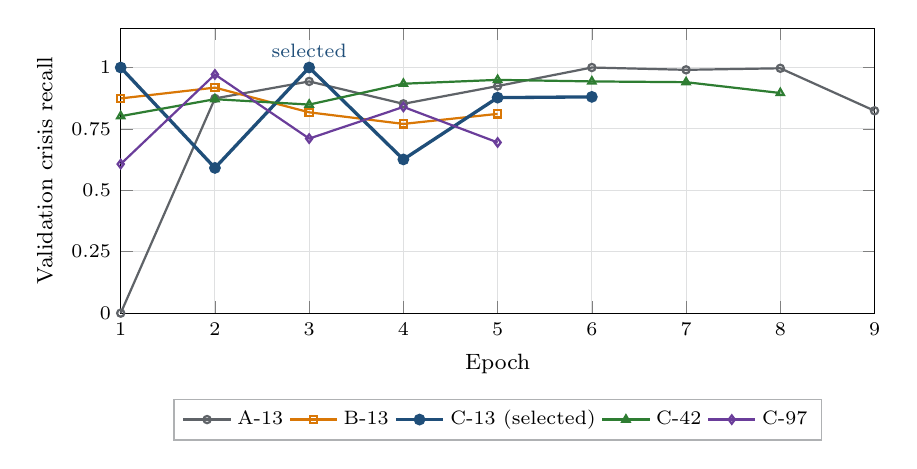
\begin{tikzpicture}
\begin{axis}[sahay, width=0.92\linewidth, height=5.2cm, clip=false,
  xlabel={Epoch}, ylabel={Validation crisis recall}, xmin=1, xmax=9, ymin=0, ymax=1.16,
  xtick={1,...,9}, ytick={0,0.25,0.5,0.75,1}, legend columns=5,
  legend style={at={(0.5,-0.30)}, anchor=north}]
\addplot[sahaygray, thick, mark=o, mark size=1.3pt] coordinates {
  (1,0.0)(2,0.8742)(3,0.9434)(4,0.8522)(5,0.9245)(6,1.0)(7,0.9906)(8,0.9969)(9,0.8239)};
\addlegendentry{A-13}
\addplot[sahayorange, thick, mark=square, mark size=1.3pt] coordinates {
  (1,0.8742)(2,0.9182)(3,0.8176)(4,0.7704)(5,0.8113)};
\addlegendentry{B-13}
\addplot[sahayblue, very thick, mark=*, mark size=1.5pt] coordinates {
  (1,1.0)(2,0.5912)(3,1.0)(4,0.6258)(5,0.8774)(6,0.8805)};
\addlegendentry{C-13 (selected)}
\addplot[sahaygreen, thick, mark=triangle, mark size=1.5pt] coordinates {
  (1,0.8019)(2,0.8711)(3,0.8491)(4,0.934)(5,0.9497)(6,0.9434)(7,0.9403)(8,0.8962)};
\addlegendentry{C-42}
\addplot[sahaypurple, thick, mark=diamond, mark size=1.5pt] coordinates {
  (1,0.6069)(2,0.9717)(3,0.7107)(4,0.8396)(5,0.695)};
\addlegendentry{C-97}
\node[font=\scriptsize, text=sahayblue, anchor=south] at (axis cs:3,1.0) {selected};
\end{axis}
\end{tikzpicture}
\caption{Validation crisis recall by epoch for the five Task 7B runs. The selected run (C-13) swings
between 1.00 and 0.59 on alternate epochs, so its selected epoch sits on a spike rather than a plateau.
C-42 is the most stable run.}
\label{fig:7bcrisis}
\end{figure}

%======================================================================
\section{Evaluation results}
\label{sec:eval}

\subsection{Task 7 checkpoint on synthetic development data (\texorpdfstring{\evB}{B})}
Table~\ref{tab:t7labels} gives per-label results for the selected checkpoint. The three weakest
labels on validation are crisis, coercion and legal urgency: crisis recall is 0.234 (Wilson 95\% CI
0.153--0.340), coercion F1 0.39, legal-urgency F1 0.40. These are the wordings the lexicon pipeline
also struggles with.

\begin{table}[!htbp]
\centering\footnotesize
\caption{Task 7 selected checkpoint (Run 2, seed 97) at the fixed 0.5 threshold. Pos.\ = positive support.}
\label{tab:t7labels}
\begin{tabular}{@{}lrcccrccc@{}}
\toprule
& \multicolumn{4}{c}{Validation (757 records)} & \multicolumn{4}{c}{Synthetic development test (843 records)} \\
\cmidrule(lr){2-5}\cmidrule(l){6-9}
Label & Pos. & Precision & Recall & F1 & Pos. & Precision & Recall & F1 \\
\midrule
Crisis / self-harm & 77 & 0.439 & \textbf{0.234} & 0.305 & 72 & 0.452 & 0.458 & 0.455 \\
Immediate danger & 86 & 0.905 & 1.000 & 0.950 & 119 & 0.943 & 0.975 & 0.959 \\
Continuing threat & 218 & 0.832 & 0.431 & 0.568 & 285 & 0.720 & 0.937 & 0.814 \\
Medical urgency & 68 & 0.850 & 1.000 & 0.919 & 97 & 0.970 & 1.000 & 0.985 \\
Isolation / boycott / displ. & 67 & 0.667 & 0.657 & 0.662 & 87 & 0.529 & 0.828 & 0.646 \\
Legal urgency & 71 & 0.550 & 0.310 & 0.396 & 76 & 0.604 & 0.724 & 0.659 \\
Coercion (comm.\ safety) & 144 & 0.358 & 0.431 & 0.391 & 151 & 0.659 & 0.894 & 0.758 \\
Explicit human request & 84 & 0.933 & 1.000 & 0.966 & 94 & 0.759 & 0.872 & 0.812 \\
\midrule
Macro (8 labels) & & 0.692 & 0.633 & 0.645 & & 0.705 & 0.836 & 0.761 \\
Micro & & 0.685 & 0.587 & 0.632 & & 0.710 & 0.874 & 0.783 \\
\bottomrule
\end{tabular}
\end{table}

\paragraph{By language.} Validation macro F1 is 0.730 in English, 0.618 in Hindi and \textbf{0.503
in Hinglish}. In both Hindi and Hinglish the minimum per-label recall is \textbf{0.00}, meaning at
least one label is never detected in those languages. On the synthetic test the figures are 0.727
(English), 0.823 (Hindi) and 0.740 (Hinglish). Code-mixed input is the hardest case, which matches
the Task~7B error analysis.

\subsection{Task 7 on the exposed regression fixtures (\texorpdfstring{\evC}{C})}
The checkpoint was run once, after selection, on the published fixtures, next to the deterministic
pipeline (Table~\ref{tab:regr}). One correction applies to the stored summaries.
The shadow micro-F1 values in the model card (0.68 dev, 0.70 candidates) include the eighth label,
explicit human request, which the deterministic pipeline does not score. Recomputed from the stored
per-label counts over the \emph{seven shared labels}, they are 0.673 and 0.683. We use the
seven-label values for comparison.

\begin{table}[!htbp]
\centering\footnotesize
\caption{Per-label F1 on the exposed fixtures (evidence class \evC; contaminated, not generalisation evidence). ``Deterministic'' is the pipeline after safety hardening. Best value per row in bold.}
\label{tab:regr}
\setlength{\tabcolsep}{4.5pt}
\begin{tabular}{@{}lcccccc@{}}
\toprule
& \multicolumn{3}{c}{Dev fixtures (57)} & \multicolumn{3}{c}{Candidate fixtures (48)} \\
\cmidrule(lr){2-4}\cmidrule(l){5-7}
Label & Deterministic & Task 7 & Task 7B & Deterministic & Task 7 & Task 7B \\
\midrule
Crisis / self-harm & \textbf{0.778} & 0.714 & 0.583 & 0.842 & \textbf{0.889} & 0.720 \\
Immediate danger & \textbf{0.933} & 0.857 & 0.333 & \textbf{1.000} & 0.727 & 0.600 \\
Continuing threat & \textbf{0.889} & 0.800 & 0.621 & \textbf{0.957} & 0.667 & 0.667 \\
Medical urgency & \textbf{1.000} & 0.800 & 0.667 & \textbf{0.800} & 0.750 & \textbf{0.800} \\
Isolation / boycott / displ. & \textbf{0.889} & 0.364 & 0.727 & 0.667 & \textbf{0.857} & 0.400 \\
Legal urgency & \textbf{1.000} & 0.462 & 0.500 & \textbf{0.923} & 0.400 & 0.571 \\
Coercion (comm.\ safety) & \textbf{0.923} & 0.400 & 0.500 & \textbf{0.571} & 0.286 & 0.462 \\
Explicit human request & \na & 0.750 & 1.000 & \na & 1.000 & 0.800 \\
\midrule
Micro F1, 7 shared labels & \textbf{0.906} & 0.673 & 0.564 & \textbf{0.868} & 0.683 & 0.622 \\
Micro F1, as stored (shadow incl.\ human req.) & --- & 0.678 & 0.585 & --- & 0.705 & 0.632 \\
Exact match & 0.860 & 0.632 & 0.544 & 0.792 & 0.667 & 0.542 \\
\bottomrule
\end{tabular}
\end{table}

\noindent The deterministic pipeline wins on 12 of the 14 label--split cells. The Task~7 shadow is
ahead only on candidate crisis (0.889 vs 0.842) and candidate isolation (0.857 vs 0.667). On the
8 red-team \emph{victim-input} cases, the Task~7 crisis firing matched expectation in 6 of 8. It
falsely fired on \code{RT-VI-EN-002} and missed the Hinglish crisis case \code{RT-VI-HG-001}.

\subsection{Task 7B on the frozen synthetic holdout (\texorpdfstring{\evB}{B}, evaluated once)}
The selected Task~7B checkpoint was evaluated \emph{once} on the 1{,}190-record frozen holdout. The
old Task~7 checkpoint was evaluated on the same holdout for comparison.

\begin{table}[!htbp]
\centering\small
\caption{Task 7B promotion gates on the frozen holdout. Any failed gate keeps the model rejected; even a full pass gives only \code{candidate\_for\_human\_review}.}
\label{tab:gates}
\begin{tabularx}{\linewidth}{@{}>{\raggedright\arraybackslash}X c >{\raggedright\arraybackslash}p{5.6cm} c@{}}
\toprule
Gate & Required & Task 7B value & Result \\
\midrule
Holdout crisis recall & $\geq 0.80$ & 1.000 (298/298; Wilson 95\% CI 0.987--1.000) & \pass \\
Crisis recall, English / Hindi / Hinglish & $\geq 0.70$ each & 1.000 / 1.000 / 1.000 & \pass \\
Legal-urgency recall & $\geq 0.70$ & 0.727 (152/209) & \pass \\
Coercion recall & $\geq 0.70$ & 1.000 (216/216) & \pass \\
Macro F1 (5 labels with support) & $\geq 0.70$ & \textbf{0.675} & \fail \\
No-alert specificity & $\geq 0.90$ & 0.925 & \pass \\
Repeat agreement & $= 1.0$ & 1.0 & \pass \\
Deterministic invariance, review packet, nothing committed & required & all true & \pass \\
Full eight-label coverage & required & \textbf{false} (3 labels with 0 positives) & \fail \\
\midrule
\multicolumn{4}{@{}l}{\textbf{Outcome:} \code{rejected\_for\_product\_integration}; human review pending} \\
\bottomrule
\end{tabularx}
\end{table}

\begin{table}[!htbp]
\centering\footnotesize
\caption{Holdout per-label results with denominators (evidence class \evB). Undefined metrics are
reported as n/a, never as 0 or 1. Also: exact match 0.773; Hamming loss 0.053; 213 false negatives and
291 false positives in total; 7 of 13 contrast groups fully correct (member accuracy 0.863).}
\label{tab:holdout}
\setlength{\tabcolsep}{4.5pt}
\begin{tabular}{@{}lrrrrcccc@{}}
\toprule
Label (Task 7B) & Pos. & TP & FP & FN & Precision & Recall & F1 & Specificity \\
\midrule
Crisis / self-harm & 298 & 298 & 66 & 0 & 0.819 & 1.000 & 0.900 & 0.926 \\
Continuing threat & 132 & 14 & 51 & 118 & 0.215 & \textbf{0.106} & 0.142 & 0.952 \\
Legal urgency & 209 & 152 & 0 & 57 & 1.000 & 0.727 & 0.842 & 1.000 \\
Coercion (comm.\ safety) & 216 & 216 & 162 & 0 & 0.571 & 1.000 & 0.727 & 0.834 \\
Explicit human request & 118 & 80 & 12 & 38 & 0.870 & 0.678 & 0.762 & 0.989 \\
Immediate danger & 0 & 0 & 0 & 0 & \na & \na & \na & 1.000 \\
Isolation / boycott / displ. & 0 & 0 & 0 & 0 & \na & \na & \na & 1.000 \\
Medical urgency & 0 & 0 & 0 & 0 & \na & \na & \na & 1.000 \\
\midrule
\multicolumn{5}{@{}l}{Macro, 5 defined labels (specificity over all 8)} & 0.695 & 0.702 & 0.675 & 0.963 \\
\multicolumn{5}{@{}l}{Micro} & 0.723 & 0.781 & 0.751 & --- \\
\bottomrule
\end{tabular}
\end{table}

\begin{figure}[!htbp]
\centering
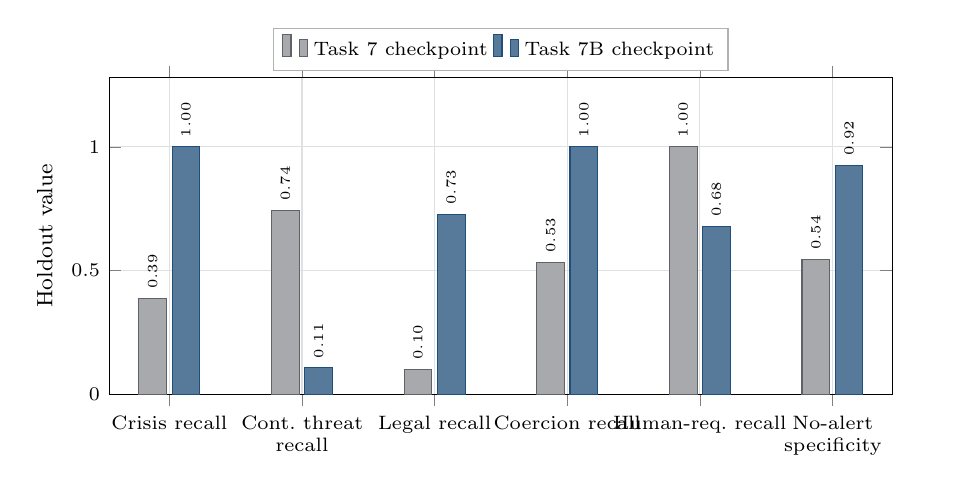
\begin{tikzpicture}
\begin{axis}[sahay, ybar, bar width=10pt, width=0.95\linewidth, height=5.6cm,
  ymin=0, ymax=1.28, ylabel={Holdout value},
  symbolic x coords={crisis,threat,legal,coercion,human,noalert},
  xtick=data,
  xticklabels={Crisis recall, Cont.\ threat recall, Legal recall, Coercion recall, Human-req.\ recall, No-alert specificity},
  x tick label style={font=\scriptsize, align=center, text width=2.2cm},
  enlarge x limits=0.09,
  nodes near coords={\pgfmathprintnumber[fixed,fixed zerofill,precision=2]{\pgfplotspointmeta}},
  nodes near coords style={font=\tiny, rotate=90, anchor=west},
  legend style={at={(0.5,1.02)}, anchor=south, legend columns=2}]
\addplot[fill=sahaygray!55, draw=sahaygray] coordinates {
  (crisis,0.3859) (threat,0.7424) (legal,0.1005) (coercion,0.5324) (human,1.0) (noalert,0.5439)};
\addplot[fill=sahayblue!75, draw=sahayblue] coordinates {
  (crisis,1.0) (threat,0.1061) (legal,0.7273) (coercion,1.0) (human,0.678) (noalert,0.9248)};
\legend{Task 7 checkpoint, Task 7B checkpoint}
\end{axis}
\end{tikzpicture}
\caption{Same holdout, two checkpoints. Task 7B fixes crisis (0.39 $\to$ 1.00), legal (0.10 $\to$ 0.73)
and coercion (0.53 $\to$ 1.00) recall and no-alert specificity (0.54 $\to$ 0.92). Continuing-threat
recall collapses from 0.74 to 0.11, and human-request recall falls from 1.00 to 0.68. On this holdout
Task 7's crisis recall was 0.51 in English, 0.38 in Hindi and 0.28 in Hinglish.}
\label{fig:holdout}
\end{figure}

\subsection{Task 7B on the exposed regression fixtures (\texorpdfstring{\evC}{C})}
Task~7B is \emph{worse} than Task~7 on the exposed fixtures (Table~\ref{tab:regr},
Figure~\ref{fig:regr}). Seven-label micro F1 fell from 0.673 to 0.564 on dev and from 0.683 to 0.622
on candidates. Crisis recall is 1.00 on both splits (7/7 and 9/9), but crisis precision is only 0.41
and 0.56 (10 and 7 false positives). On the red-team victim-input cases it matched 7 of 8; the
Hinglish crisis case \code{RT-VI-HG-001} is still missed.

\begin{figure}[!htbp]
\centering
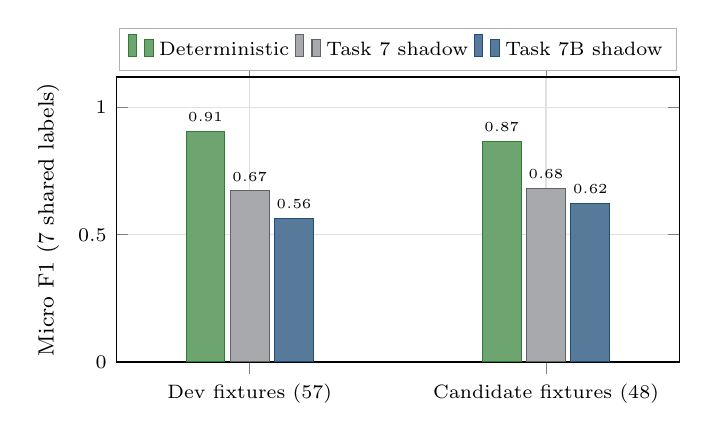
\begin{tikzpicture}
\begin{axis}[sahay, ybar, bar width=14pt, width=0.72\linewidth, height=5.2cm,
  ymin=0, ymax=1.12, ylabel={Micro F1 (7 shared labels)},
  symbolic x coords={dev,cand}, xtick=data,
  xticklabels={Dev fixtures (57), Candidate fixtures (48)},
  enlarge x limits=0.45,
  nodes near coords={\pgfmathprintnumber[fixed,fixed zerofill,precision=2]{\pgfplotspointmeta}},
  nodes near coords style={font=\tiny},
  legend style={at={(0.5,1.02)}, anchor=south, legend columns=3}]
\addplot[fill=sahaygreen!70, draw=sahaygreen] coordinates {(dev,0.906) (cand,0.8675)};
\addplot[fill=sahaygray!55, draw=sahaygray] coordinates {(dev,0.6729) (cand,0.6829)};
\addplot[fill=sahayblue!75, draw=sahayblue] coordinates {(dev,0.5641) (cand,0.6222)};
\legend{Deterministic, Task 7 shadow, Task 7B shadow}
\end{axis}
\end{tikzpicture}
\caption{Contaminated exposed regression (evidence class \evC). Task 7B improves on the synthetic
holdout and gets worse on the human-written fixtures: it fits the generator, not the task.}
\label{fig:regr}
\end{figure}

\subsection{Deterministic invariance and reproducibility}
Invariance is the property that matters most for safety: whatever the shadow model does must not
change the authoritative pipeline. Sixty records were each run under seven shadow conditions: the
real model, always fires, always silent, raises an error, times out, returns malformed output, and
missing. The deterministic outputs were identical in every case (0 mismatches). Repeat agreement of
the shadow model was 1.0, and every Stage~C seed reproduced identical predictions on re-run.

\subsection{The authoritative deterministic pipeline}
\label{sec:det}
The deterministic text pipeline has its own evaluation. It uses no model, no network and no LLM
(Table~\ref{tab:det}). The baseline (2026-09-11) used crisis lexicon \code{crisis-v1.1} and
validator \code{guardrails-v1}. The hardening round moved to \code{crisis-v1.2},
\code{guardrails-v1.1} and 87 output rules. The SVI scoring version \code{svi-2026.09-pc08} was
unchanged.

\begin{table}[!htbp]
\centering\footnotesize
\caption{Deterministic detectors at baseline (precision / recall / F1). Explicit human request is excluded (button, not text).}
\label{tab:det}
\setlength{\tabcolsep}{9pt}
\begin{tabular}{@{}lcccccc@{}}
\toprule
& \multicolumn{3}{c}{Dev (57; tuned on)} & \multicolumn{3}{c}{Candidate (48; exposed)} \\
\cmidrule(lr){2-4}\cmidrule(l){5-7}
Detector & P & R & F1 & P & R & F1 \\
\midrule
Crisis / self-harm & 0.636 & 1.000 & 0.778 & 0.714 & 0.556 & 0.625 \\
Immediate danger & 1.000 & 0.875 & 0.933 & 1.000 & 1.000 & 1.000 \\
Continuing threat & 1.000 & 0.800 & 0.889 & 1.000 & 0.917 & 0.957 \\
Medical urgency & 1.000 & 1.000 & 1.000 & 1.000 & 0.667 & 0.800 \\
Isolation / boycott / displ. & 1.000 & 0.800 & 0.889 & 1.000 & 0.500 & 0.667 \\
Legal urgency & 1.000 & 1.000 & 1.000 & 1.000 & 0.857 & 0.923 \\
Coercion (comm.\ safety) & 1.000 & 0.857 & 0.923 & 1.000 & 0.400 & 0.571 \\
\bottomrule
\end{tabular}
\end{table}

\begin{table}[!htbp]
\centering\small
\caption{Headline safety metrics, baseline vs.\ after hardening. Candidate numbers after hardening are regression numbers, because the failures were read while designing the fixes.}
\label{tab:dethard}
\begin{tabular}{@{}lcccc@{}}
\toprule
& \multicolumn{2}{c}{Baseline} & \multicolumn{2}{c}{After hardening} \\
\cmidrule(lr){2-3}\cmidrule(l){4-5}
Metric & Dev & Candidate & Dev & Candidate \\
\midrule
Critical misses / events & 1/17 & 4/14 & 1/17 & 1/14 \\
\quad Wilson 95\% CI of miss rate & 0.010--0.270 & 0.117--0.547 & 0.010--0.270 & 0.013--0.315 \\
False escalations & 2 & 2 & 2 & 2 \\
Crisis pre-check P / R & 0.636 / 1.000 & 0.714 / 0.556 & 0.636 / 1.000 & 0.800 / 0.889 \\
Evidence validity (cited turns real) & 1.000 & 1.000 & 1.000 & 1.000 \\
Guardrail red-team (39 cases) & \multicolumn{2}{c}{20/39 pass} & \multicolumn{2}{c}{39/39 pass (exposed)} \\
Near-miss / leakage development cases & \multicolumn{2}{c}{---} & \multicolumn{2}{c}{75/75 and 29/29 pass} \\
\bottomrule
\end{tabular}
\end{table}

\noindent Remaining failures:
\begin{itemize}
  \item two critical misses, \code{DEV-EN-022} and \code{CAND-EN-003};
  \item four false escalations, \code{DEV-EN-011}, \code{DEV-HI-012}, \code{CAND-EN-012} and
        \code{CAND-HI-009}, all from crisis wording that is quoted or attributed to someone else;
  \item detector false negatives concentrated in coercion, isolation and continuing threat.
\end{itemize}
The MVP target M1 (zero critical misses on the scripted corpus) is \textbf{not met}. The SVI
sensitivity analysis found four things:
\begin{itemize}
  \item without a hard override, the highest text-only SVI is 71.8 (High);
  \item D2 is binary in text, so its 0.18 weight never moves a band on its own;
  \item seven weak tier-1 signals can reach 50.91 (Moderate) with no strong indicator;
  \item repeated future threats stay at or below 69, under the override threshold of 70.
\end{itemize}
The reproducibility checks all passed: two runs were identical, the 10 multi-turn replays were
consistent, the LLM-off walk validated all 16 fallbacks, and no network attempt was made.

\paragraph{External exploratory firing rates.} The deterministic pipeline was also run on private
samples of the external datasets. These rates are \emph{not} correctness measures, because no SAHAY
label exists for these records:
\begin{itemize}
  \item \textbf{Reddit Suicide Detection:} the crisis pre-check fired on 53.9\% of records from the
        suicide subreddit and 1.6\% of the others.
  \item \textbf{Dreaddit:} 3.0\% on stressed records vs.\ 1.7\% on unstressed ones.
  \item \textbf{EmoInHindi:} the legal-urgency detector fired on 51.6\% of records and medical
        urgency on 23.8\%. That fits the corpus's legal and mental-health counselling domain; it
        is not evidence of overbreadth.
  \item \textbf{Hinglish hate speech and sentiment:} essentially nothing fired (0.0--0.1\%).
\end{itemize}

\subsection{Model runtime qualification (Task 6)}
\label{sec:runtime}
Task~6 measured latency and memory only, on fictional text and synthetic signals
(Table~\ref{tab:runtime}). None of these numbers is a quality measurement. Real Hindi and English
WER is \textbf{unmeasured} until approved, transcribed evaluation audio exists.

\begin{table}[!htbp]
\centering\footnotesize
\caption{Runtime on the RTX 4060 laptop (fp16 CUDA unless stated). p50 over 20 runs (encoders, VAD) or 5 runs (ASR).}
\label{tab:runtime}
\begin{tabularx}{\linewidth}{@{}>{\raggedright\arraybackslash}p{3.3cm}X@{}}
\toprule
Component & Measurement \\
\midrule
MuRIL (primary encoder) & Cold load 7.8\,s. Encode p50 at 128 tokens: 17.8\,ms (en), 14.8\,ms (hi), 16.3\,ms (Hinglish); 327--397 samples/s at batch 8. Tokens per character: 0.209 / 0.246 / 0.259; unknown-token rate 0. Peak 504\,MB. \\
XLM-R (comparison only) & Cold load 4.2\,s. Encode p50 at 128 tokens: 15.9 / 19.0 / 15.9\,ms. Tokens per character: 0.232 / 0.319 / 0.294. \\
Whisper Small (faster-whisper, CTranslate2) & Cold load 1.1\,s. On a speech-like \emph{synthetic} signal: 5\,s English 523\,ms (real-time factor 0.105); 5\,s Hindi 2{,}349\,ms (RTF 0.47); 30\,s Hindi 2{,}365\,ms (RTF 0.08). Hindi decoding takes about 2.35\,s whatever the clip length, which suggests the decoder runs to a length limit on non-speech. \\
Silero VAD (CPU) & p50 98\,ms for 5\,s of audio, 595\,ms for 30\,s, 1{,}186\,ms for 60\,s (about 20\,ms per audio second). \\
Gated pipeline & 10\,s of silence: 0 speech intervals, Whisper never invoked, 225\,ms in total. \\
Ungated worst case (benchmark only) & Forced to decode 5\,s of \emph{silence} in Hindi, Whisper produced a median 186 characters of fluent text; a pure tone produced 148 characters. English: 3 and 0. \\
Coexistence & MuRIL and Whisper together use 1{,}102\,MB of device memory, leaving 5{,}950\,MB of headroom on 8\,GB. \\
\bottomrule
\end{tabularx}
\end{table}

\noindent The worst-case row is why Silero VAD is an \emph{enforced} precondition rather than an
optimisation. \code{WhisperASR.transcribe} has no default for its speech intervals, validates them
before decoding, and skips Whisper when no speech is found. A VAD false positive can still reach
Whisper, and that remains a documented risk.

%======================================================================
\section{Discussion}
\label{sec:discussion}

\paragraph{1. Domain adaptation worked as language modelling; its downstream value is unproven.}
Stage~A cut held-out perplexity by 48\%, and the Stage~B heads show the adapted encoder separates
several source tasks. But no ablation was run against un-adapted MuRIL, XLM-R, or the planned
LogReg and XGBoost baselines. The Stage~C results therefore cannot be attributed to Stage~A.

\paragraph{2. The synthetic-to-real gap dominates.}
On the \emph{same} frozen holdout, Task~7B raised micro F1 from 0.50 to 0.75. On the human-written
exposed fixtures it \emph{lost} ground: 7-label micro F1 fell from 0.673 to 0.564 on dev. The most
plausible reading is that the head learns the style of the template generator. A holdout drawn from
the same generator family is not a proxy for real performance, however carefully it is frozen.

\paragraph{3. Crisis recall was bought with continuing-threat recall.}
Continuing-threat positives fell from 1{,}667 in the Task~7 training set to 453 in Task~7B's.
Task~7B's selection rule ranks crisis recall first and, through the ``weak-label'' minimum, only
legal and coercion recall after it. Continuing threat enters only through macro F1. The result is a
recall collapse from 0.74 to 0.11 on that label (Wilson 95\% CI 0.064--0.170). Crisis selection was
also volatile: the chosen epoch sits on a spike (Figure~\ref{fig:7bcrisis}).

\paragraph{4. Split design matters as much as the model.}
Splitting by family put \emph{all} positives for immediate danger, isolation and medical urgency
into training, leaving validation and holdout with none. The metric-validity correction made this
visible: it reports those labels as undefined rather than zero-filling them and flatters nothing.
Any future corpus must stratify family assignment by label.

\paragraph{5. The deterministic pipeline is precise but brittle.}
Its precision is 1.0 on almost every detector. Its failures are recall gaps on paraphrase,
coercion and isolation wording, plus false escalations from quoted crisis language. A learned model
could help as a \emph{recall-oriented second opinion} for an officer. Task~7B's crisis recall of
1.00 on both exposed splits hints at this, but its precision (0.41--0.56) and the persistent
Hinglish miss (\code{RT-VI-HG-001}) show it is not ready even for that role.

\paragraph{6. Relation to the literature.}
Refs.~\cite{hu2024,islam2024} report 89--97.5\% accuracy for binary PTSD or emotion tasks on small or
acted datasets. SAHAY-AI's task is different: multi-label, multilingual, code-mixed, and reported
under strict evidence separation. It gives far more modest numbers, and says so. The weak severity
signal in~\cite{hu2024} ($R^2=0.10$) supports the decision not to derive severity from voice. MuRIL's
transliteration advantage~\cite{khanuja2021} is reflected in our tokeniser measurements, yet
code-mixed Hinglish remains the hardest input: it has the lowest Task~7 validation macro F1 (0.50)
and the lowest Task~7 holdout crisis recall (0.28). EmoInHindi~\cite{singh2022} is domain-relevant, but its
emotion labels, and the Stage~B head's failure on \emph{fear}, confirm that emotion is not a
vulnerability proxy.

\paragraph{7. Governance held.}
Several practices worked as designed:
\begin{itemize}
  \item the plan was hashed before training, and the corpus frozen;
  \item the holdout was evaluated only once;
  \item metrics carry denominators, and undefined values stay undefined;
  \item evidence classes were never pooled;
  \item the source-label firewall held, and shadow isolation was verified by the invariance test.
\end{itemize}
Together they turned a disappointing model into a trustworthy negative result, the outcome the
project's safety invariants are built to allow.

%======================================================================
\section{Limitations and threats to validity}
\label{sec:limits}
\begin{itemize}
  \item \textbf{No official or independent evaluation.} The locked set has 0 samples, and no blind
        corpus has been authored or frozen. Every number is class \evB{} or \evC.
  \item \textbf{Synthetic supervision.} The SAHAY labels come from agent-written templates. None of
        the 2{,}266 review-packet items has been reviewed by a person.
  \item \textbf{Small fixture sets.} With 17 and 14 critical events, a single miss moves the miss
        rate by 6--7 points. The Wilson intervals in Table~\ref{tab:dethard} span 0.01--0.27 and
        0.01--0.32.
  \item \textbf{Uncalibrated threshold.} The fixed 0.5 threshold is a convention, not an operating
        point. No calibration, reliability diagrams or AUPRC were computed, though the handover
        plan lists them.
  \item \textbf{Unresolved data rights.} Licensing and privacy approval for the Stage~A datasets
        are unresolved. They contain real user-generated text, may include minors, and names are not
        reliably redacted. If a review refuses a dataset, the derived checkpoints must be
        quarantined.
  \item \textbf{Voice is unevaluated.} ASR quality (WER) is unmeasured, D4 is unavailable, and
        Whisper hallucination is mitigated but not eliminated.
  \item \textbf{Single machine and seed sensitivity.} Runtime numbers come from one laptop GPU.
        Stage~C results vary by 0.07 or more in macro F1 across seeds.
  \item \textbf{Literature numbers were not reproduced.} The results of~\cite{hu2024,islam2024}
        are quoted from their abstracts, not replicated.
\end{itemize}

%======================================================================
\section{Recommendations and next steps}
\label{sec:next}
\begin{enumerate}
  \item \textbf{Build the independent evaluation first.} Recruit human authors and reviewers through
        \code{ml/eval/blind/}, freeze a blind corpus, and fill the locked set, with two reviewers on
        every crisis and immediate-danger sample. Until then, no model claim can move beyond
        development evidence.
  \item \textbf{Complete the human review packet} (2{,}266 items) before any promotion decision.
  \item \textbf{Fix corpus coverage.} Stratify family splits so every label has positive and
        negative support in validation and holdout. Restore continuing-threat support. Treat the
        \code{7b-v1} holdout as exposed and version a new one.
  \item \textbf{Add the missing controls:} un-adapted MuRIL, XLM-R, and the planned LogReg and
        XGBoost baselines, all under the same protocol.
  \item \textbf{Stabilise selection.} Select on a smoothed or plateau criterion, not a single-epoch
        spike. Report per-label AUPRC and calibration; choose any threshold on validation only.
  \item \textbf{Resolve data rights} for the Stage~A datasets, or retrain Stage~A without the
        unresolved ones, and record the decision.
  \item \textbf{Measure ASR} on approved, transcribed Hindi and English audio (EXT-002). Benchmark
        IndicConformer~\cite{ai4bharat} only after its own approval.
  \item \textbf{Prepare for DPDP commencement} (consent-manager provisions around November 2026,
        substantive obligations around May 2027), with a legal review of notices, retention and
        breach handling~\cite{meity2023}.
\end{enumerate}

%======================================================================
\section{Conclusion}
The references establish that speech and text carry trauma-relevant signal~\cite{hu2024,islam2024},
that NHAA 14566 needs multilingual, round-the-clock, docketed intake~\cite{pib2021}, and that India's
data-protection regime is arriving in phases~\cite{meity2023}. They also point to the right open
tools: MuRIL, IndicConformer, faster-whisper and EmoInHindi~\cite{khanuja2021,ai4bharat,systran,singh2022}.

The team's trained model, a MuRIL-based eight-label shadow classifier, shows that domain adaptation
works as language modelling. It also shows that targeted synthetic data can drive crisis recall to
1.00 on a synthetic holdout. But it does not generalise to human-written fixtures, it trades one
safety label for another, and it cannot be fully evaluated on its own holdout. It therefore remains
\code{rejected\_for\_product\_integration}.

The deterministic pipeline stays the authority, with two known critical misses on the exposed
fixtures and an honest record of every failure. The next milestone is not a better model but an
independent, human-authored evaluation set. Without one, no model in this project can earn trust.

%======================================================================
\appendix
\section{Reproducibility and provenance}
\label{app:repro}

\begin{table}[!htbp]
\centering\footnotesize
\caption{Pinned artefacts and hashes (weights, corpora and reports stay private beneath \code{SAHAY\_TRAINING\_ROOT}; never committed).}
\begin{tabularx}{\linewidth}{@{}>{\raggedright\arraybackslash}p{4.0cm}>{\raggedright\arraybackslash}X@{}}
\toprule
Artefact & Identifier \\
\midrule
Base encoder & \code{google/muril-base-cased} @ \code{afd9f36c7923d54e97903922ff1b260d091d202f} (Apache-2.0) \\
ASR & \code{openai/whisper-small} @ \code{973afd24\ldots}, converted locally to CTranslate2 fp16; faster-whisper 1.2.1, CTranslate2 4.8.2 \\
VAD & \code{silero-vad} 6.2.1 \\
Stage A run & \code{run-20260912-054730}; \code{model.safetensors} sha256 \code{550fc3a2\ldots a35c}; corpus \code{external-ext119-v1}, segments sha256 \code{37f5bf5d\ldots f844} \\
Task 7 selected checkpoint & \code{stage-c/run2-seed-97}; fictional corpus sha256 \code{f07cfbfa\ldots 97e3}; template bank \code{9cb89828\ldots 78b0} \\
Task 7B plan & sha256 \code{843f3e2c62545e79\ldots 892b}, recorded 2026-09-12 11:06:48 IST \\
Task 7B corpus \code{7b-v1} & frozen 2026-09-12 11:01:49 IST; template bank \code{43ac65f9\ldots bb43}; holdout sha256 \code{3fad8607\ldots eb22} \\
Task 7B selected checkpoint & \code{task7b/checkpoints/C-seed-13}, epoch 3 \\
Software & Python 3.12, torch 2.11.0+cu128, transformers 5.17.0, tokenizers 0.23.2, accelerate 1.15.0, safetensors 0.8.0, numpy 2.5.3 \\
\bottomrule
\end{tabularx}
\end{table}

\paragraph{Commands} (private model environment, offline with sockets blocked, explicit
\code{SAHAY\_DATASETS\_ROOT}, \code{SAHAY\_MODELS\_ROOT} and \code{SAHAY\_TRAINING\_ROOT}):

\begin{tcolorbox}[enhanced,colback=sahaygray!5,colframe=sahaygray!40,boxrule=0.4pt,arc=1pt,left=4pt,right=4pt,top=2pt,bottom=2pt]
\footnotesize\ttfamily
python -m ml.data.training\_corpus build --ext119-local-training --acknowledge "<EXT-119 sentence>"\\
python -m ml.training.cli preflight | fictional | stage-a | stage-b\\
python -m ml.training.cli stage-c --seeds 13 42 97 --epochs 20 --patience 3 --tag run2\\
python -m ml.training.cli verify-shadow | regression | error-analysis\\
python -m ml.training.cli hardening-build | hardening-verify | stage-c7b-plan\\
python -m ml.training.cli stage-c7b --phase 1 | stage-c7b --phase 2 | stage-c7b-select\\
python -m ml.training.cli stage-c7b-evaluate | stage-c7b-correct\\
python -m ml.eval.run\_eval \quad\# deterministic evaluation (standard library only)\\
python -m ml.eval.hardening\_report
\end{tcolorbox}

\paragraph{Project-internal sources used for this report.}
\begin{itemize}[itemsep=0pt]
  \item Repository: \filepath{ml/training/README.md}, \filepath{ml/shadow/MODEL_CARD.md},
        \filepath{ml/eval/README.md}, \filepath{ml/runtime/README.md},
        \filepath{ml/data/cards/emoinhindi.md}.
  \item Baseline evaluation: \filepath{ml/eval/results/eval-baseline-2026-09-11.md}.
  \item Hardening report: \filepath{ml/eval/results/safety-hardening-2026-09-11.md}.
  \item Specification and decisions: \filepath{docs/HANDOVER.md} and
        \filepath{docs/EXTERNAL_DECISIONS.md} (EXT-118 to EXT-121).
  \item Private reports under \filepath{sih-dataset/training/} and \filepath{sih-dataset/reports/}.
        They hold aggregate JSON only; no record text was read for this report.
\end{itemize}

\section{Label definitions}
\label{app:labels}
\begin{table}[!htbp]
\centering\footnotesize
\caption{The eight detector categories (label schema 1.0.0) and the deterministic signal each is judged on.}
\begin{tabularx}{\linewidth}{@{}>{\raggedright\arraybackslash}p{3.6cm}>{\raggedright\arraybackslash}p{4.9cm}>{\raggedright\arraybackslash}X@{}}
\toprule
Category & Code identifier & Deterministic signal \\
\midrule
Crisis / self-harm & \code{crisis\_self\_harm} & The synchronous crisis pre-check fires on the turn \\
Immediate danger & \code{immediate\_danger} & A D1 tier-3 (imminent presence) lexicon match \\
Continuing threat & \code{continuing\_threat} & Any D1 match, or a D3 match of tier 2 or above \\
Medical urgency & \code{medical\_urgency} & A D7 match of tier 2 or above (pain alone is tier 1) \\
Isolation / boycott / displacement & \code{isolation\_boycott\_displacement} & Any D6 match \\
Legal urgency & \code{legal\_urgency} & Any D8 match \\
Coercion (communication safety) & \code{communication\_safety\_coercion} & Any D9 match, or evidence behind the coercion alert \\
Explicit human request & \code{explicit\_human\_request} & Excluded: the app sends \code{request\_human} from a button \\
\bottomrule
\end{tabularx}
\end{table}

\noindent A \emph{critical miss} is a sample whose expected routing is Critical but that was neither
caught by the pre-check nor banded Critical. A \emph{false escalation} is a sample routed Critical
when it should not have been. Labels describe what the text \emph{means}, not what the system does.
A crisis phrase quoted in someone else's words is labelled \code{crisis\_self\_harm = false}.

%======================================================================
\begin{thebibliography}{9}
\setlength{\itemsep}{3pt}
\small

\bibitem{hu2024}
J.~Hu, C.~Zhao, C.~Shi, Z.~Zhao and Z.~Ren.
Speech-based recognition and estimating severity of PTSD using machine learning.
\emph{Journal of Affective Disorders}, 362:859--868, 2024.
\url{https://doi.org/10.1016/j.jad.2024.07.015}

\bibitem{islam2024}
K.~Islam and Z.~ElSayed.
Speech-based emotion recognition and PTSD detection through machine and deep learning.
\emph{International Journal of Computer Engineering in Research Trends (IJCERT)}, 11(3):46--53, 2024.
doi:10.22362/ijcert/2024/v11/i3/v11i306.
\url{https://www.ijcert.org/index.php/ijcert/article/view/978/861}

\bibitem{pib2021}
Ministry of Social Justice and Empowerment, Press Information Bureau.
14566 --- National Helpline Against Atrocities on SCs/STs. Press release, December 2021.
\url{https://pib.gov.in/Pressreleaseshare.aspx?PRID=1780741}

\bibitem{meity2023}
Ministry of Electronics and Information Technology (MeitY), Government of India.
The Digital Personal Data Protection Act, 2023, and the Digital Personal Data Protection Rules, 2025.
\url{https://www.meity.gov.in}

\bibitem{khanuja2021}
S.~Khanuja, D.~Bansal, S.~Mehtani, S.~Khosla, A.~Dey, B.~Gopalan, D.~K.~Margam, P.~Aggarwal,
R.~T.~Nagipogu, S.~Dave, S.~Gupta, S.~C.~B.~Gali, V.~Subramanian and P.~Talukdar.
MuRIL: Multilingual representations for Indian languages.
arXiv:2103.10730, 2021.
\url{https://arxiv.org/abs/2103.10730}

\bibitem{ai4bharat}
AI4Bharat.
IndicConformer: multilingual ASR for the 22 official Indian languages. Software repository.
\url{https://github.com/AI4Bharat/IndicConformerASR}

\bibitem{systran}
SYSTRAN.
faster-whisper: faster Whisper transcription with CTranslate2. Software repository.
\url{https://github.com/SYSTRAN/faster-whisper}

\bibitem{singh2022}
G.~V.~Singh, P.~Priya, M.~Firdaus, A.~Ekbal and P.~Bhattacharyya.
EmoInHindi: A multi-label emotion and intensity annotated dataset in Hindi for emotion recognition
in dialogues. In \emph{Proceedings of the Thirteenth Language Resources and Evaluation Conference
(LREC 2022)}, pages 5829--5837, Marseille, France, 2022.
\url{https://aclanthology.org/2022.lrec-1.627/}

\end{thebibliography}

\noindent{\footnotesize\color{sahaygray} All URLs accessed 13 September 2026. PIB and MeitY pages
refused automated access (HTTP 403); their content was verified through the PIB mirror and public
summaries of the gazette notification.}

\end{document}
